%%%%%%%%%%%%%%%%%%%%%%%%%%%%%%%%%%%%%%%%%
% SC Information Paper 5 
% SHARK INDICATORS IN THE WESTERN CENTRAL PACIFIC
% June 2015
%
% Author: Joel Rice (joelrice@uw.edu )
%
%
%%%%%%%%%%%%%%%%%%%%%%%%%%%%%%%%%%%%%%%%%

%----------------------------------------------------------------------------------------
%  PACKAGES AND OTHER DOCUMENT CONFIGURATIONS
%----------------------------------------------------------------------------------------
\documentclass[12pt]{SCreport}

\graphicspath{ {C:/Projects/SHK-indicators-2015/GRAPHICS/} {C:/Projects/SHK-indicators-2015/GRAPHICS/Defined/} {C:/Projects/SHK-indicators-2015/GRAPHICS/CPUE_std/} }

\usepackage[english]{babel}


%\documentclass[12pt]{SCreport}
\newtoggle{includefigs}
%\togglefalse{includefigs} % to include figures, uncomment \toggletrue{includefigs} 
%\usepackage{graphicx} 
\usepackage{multirow} 
\usepackage{array} 
%\usepackage{lscape} 
%\usepackage{caption} 
\usepackage{subcaption}

\toggletrue{includefigs}


  \reportauthor{Joel Rice\footnote{Joel Rice Consulting Ltd.}, Laura Tremblay-Boyer, and Shelton Harley}
  \reporttitle{Analysis of stock status and related indicators for key shark species of the Western Central Pacific Fisheries Commission}
  \reportnumber{SA-IP-05}

\usepackage{grffile}

%----------------------------------------------------------------------------------------
%  Document content
%----------------------------------------------------------------------------------------

\begin{document}

\wcpfctitlepage

\tableofcontents

%\section{Executive Summary}

\section{Introduction} % ltb rev 90% done

% This study provides indicators related to the stocks general trend, whether it has changed from the previous indicator analysis and if further analysis is warrented, how to undertake that analysis.  Uncertainty regarding any species population level mechanisims that drive any indivudal anlysis is qualitiatively expressed  by species and stock in order to represent the uncertainty in the underlying data. 

Sharks are typically caught as bycatch in the Pacific tuna fisheries, though some directed and/or mixed species fisheries also exist. The status of the shark species designated as key shark species in 2011 (blue, mako, thresher, silky oceanic whiteip  sharks) in the Western and Central Pacific Ocean (WCPO) \hl{ADD REF} underwent a comprehensive review in 2011 \citep{Clarke2011_a}. That review presented a number of indicators to inform on the status of the stock of these shark species and their response to fishing pressure. Given the paucity of data availability for shark species compared to target species, the indicators they developed were based on the type of information typically available from operational-level data for industrial purse-seine and longline fleets. 

The current study updates key indicators and extends previous analyses to include hammerhead, porbeagle and whale sharks.  

In this report, we present information on the geographic range of catches for each of the species considered; temporal trends in catch composition and catch rates, and key biological indicators of fishing pressure such as mean size and sex ratio by species. Whale sharks are assessed separately due to the unique nature of their interactions with fisheries in the WCPO. The analyses are based on Secretariat of the Pacific Community - Oceanic Fisheries Programme (SPC-OFP) data holdings for sharks taken in longline and purse seine fisheries in the WCPO.  Our analysis generally follows the framework first developed and described in the Shark Research Plan presented to the sixth meeting of the Western and Central Pacific Fisheries Commission's (WCPFC) Scientific Committee (SC6; Clarke and Harley 2010). 

\subsection{Report layout}
This report is necessarily large. To assist the reader it has been structured along the following lines. Following a brief description of the available data in section 2, each of the four indicator analyses are described and results summarized in sections 3-6. Section 7 presents a consideration of the feasibility of conducting a formal stock assessment for each of the shark species discussed in this report.  In Section 8, we review the impact of recent shark management measures and, in section 9, recommend future work to extend and improve the indicator analysis approach.  Conclusions arising from our analysis of stock indicators are summarized in section 10.  Finally, section 11 discusses the management implications arising from the results of the work presented here.

\section{Description of Data}

The primary source of catch information regarding sharks is the SPC-held observer database which, despite low coverage in all regions (Table \ref{tbl:obscov}), has a substantial amount of information regarding operational characteristics as well as fate and condition data on captured sharks. Our measure of observer coverage is defined by "observed hooks set" and is used here because it is a "common currency" and allows for the standardisation of observer coverage rates when undertaking analyses.  In addition to the observer data, SPC holds operational logsheet and aggregate data on shark catches by longline fisheries. The operational data submitted to the SPC are at a higher spatial resolution than the aggregate data, and are useful for catch estimation, but in practice their utility is limited by the lack of data provision by species for shark (Table \ref{tbl:logcov}), especially in equatorial regions where the majority of the longline effort occurs. This study covers the time period 1995-2014. While some observer and logbook data exist for years prior to 1995, the majority of records either do not report shark catch or list it as a general category 'shark'.  At the time of analysis, sufficient data for 2014 was available both in logsheets and the observer data, notable exceptions from the observer database for 2014 are Australia and the United States whose most recent contributions were in 2011.
%JR
%The primary source of catch information regarding sharks is the SPC held observer data which, despite low coverage in all regions (Table 1 -\%Observer coverage by region) has a significant amount of information regarding operational characteristics as well as the fate and condition of sharks caught. In addition to the observer data, SPC holds operational logsheet and aggregate data on shark catches by longline fisheries. The operational data submitted to the SPC are at a higher spatial resolution, and are useful for catch estimation, but in practice the utility is limited by the lack of data provision by species for shark \hl{(Table 2 Logsheet coverage by region \% that ID sharks to species)}, especially in equatorial regions where the majority of the longline effort occurs
%(\ref{fig:regions}).

Aggregate coverage rates are on par with the coverage rates of the operational logsheet data sets, although coverage differs greatly by region (\hl{Table 3 - NO SUCH TABLE CURRENTLY}). Historical coverage rates are poor partly because prior to February 2011 sharks were not amongst the species for which data provision was required (WCPFC 2013); since that time, data provision for the 13 species designated by WCPFC as key shark species is mandatory . Under CMM 2007-01, required levels of Regional Observer Programme (ROP) coverage in longline fisheries are set to rise to 5\% from June 2012 in most areas, but annual average values have been $\leq$1\% in recent years (for the entire WCPO). With some notable exceptions (e.g. northeast and southwest of Hawaii), most observed sets occurred within Exclusive Economic Zones (EEZs). A thorough examination of the SPC-held fisheries data and its utility for shark related analyses can be found in Clarke et al. (2011).

Building on the work of Clarke et al (2011), this indicator analysis uses the six WCPFC statistical areas as defined in the 2010 WCPFC bigeye tuna stock assessment (Figure \ref{fig:fig01}). As noted in Clarke et al. (2011), these regions are somewhat arbitrarily assigned to the key shark species. However, given the fact that the predominant source of fishing mortality for these species is the longline fishery targeting tropical tunas (as well as billfishes and occasionally sharks), these regions adequately capture the important characteristics of the fisheries. Therefore, for purposes of comprehension and comparison to the previous analysis, we opted to keep the same regions. We note that the current bigeye tuna assessment utilizes a set of regions that differs from those used here, however as the change is to subdivide a few of the large regions, and to maintain comparability with previous analyses, we opted to work with the six-region set presented here.


%\addcenterfig]{}{P}

\begin{figure}
\begin{center}
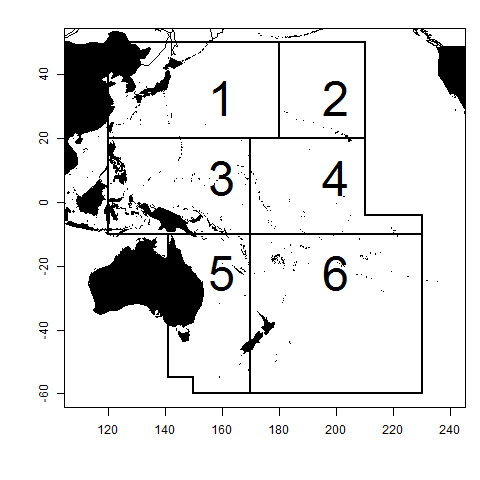
\includegraphics[scale=0.95]{../GRAPHICS/Defined/FIG_01_MAP}
\caption{\label{fig:fig01} Map of WCPO and regions used for the analysis.}
\end{center}
\end{figure}

%----------------------------------------------------------------------------------------

\subsection{Longline Fishery Data}
%---------------------------------------------------------------------------------------------
  
Longline fishing effort in the WCPO has increased steadily over the study period (1995-2014) to approximately 800 million hooks, with nearly half of the effort occurring in Regions 3 and 4 (Table \ref{tab:hooksfished}).  Ideally, indicator analyses would be based on operational-level data as its higher spatial resolution permits more comprehensive and nuanced analyses, however SPC's operational level data is geographically limited with respect to provision of shark data.  Figure \ref{fig:fig02} illustrates the geographic distribution of sets for which SPC holds operational data (blue dots) and sets with at least one recorded shark are overplotted (in orange). However, this picture is somewhat misleading as only 41\% of the operational-level sets plotted recorded any sharks. This is in contrast to the observer data in which 93\% of the sets recorded at least one shark (overplotted in red).

This is not necessarily due to misreporting. Prior to February 2011, sharks were not amongst the species for which data provision was required (WCPFC 2011); since that time data provision for the 13 species designated by WCPFC as key shark species has been mandatory. Figure \ref{fig:fig02} does not distinguish between key shark species and other shark species because only 16\% of the reported sets recorded any species-specific shark catches. Clarke et al. (2011b) note that most historical species-specific shark catch data are provided by a small number of flag States.

Given the relatively low level of coverage in the operational-level logsheets, a more complete characterization of the longline fishery requires the use of the SPC-held aggregated (5\degree x 5\degree grid) data. Effort and reported shark catch data by flag at the aggregated level have a lower degree of spatial resolution but in most cases are raised to represent the entire WCPO longline fishery. Sets with observers present onboard, are shown for comparison (Figure \ref{fig:fig03}) but have a finer degree of spatial resolution due to observer record keeping. 

A comparison of longline effort by flag and the number of sharks recorded in logsheets was constructed (Figure \ref{fig:fig04}) by showing the top four fishing nations (in the WCPO as a whole) and aggregating the rest of the flag states to another group. If the fishing practices and reporting practices were more or less consistent across flags the numbers of sharks reported would be proportional, by flag, to the effort.

Comprehensive data on shark catches at high spatial resolution are available from observer data held by the SPC-OFP but, as described above, the overall coverage of these data is low, and much less than the required levels of ROP coverage. In addition, a comparison of longline effort and longline observer coverage (Figure \ref{fig:fig05}) reveals that the latter is disproportional by region and flag and thus cannot be considered representative of the fishery as whole.

Another aspect of the low data coverage problem is that of temporal representativeness on a month/year basis of the observed effort. A comparison of the annual proportion observed by month - on a regional basis - shows significant fluctuations in the relative coverage of the observer data compared to the logbook data (Figure \ref{fig:fig06}).

\begin{comment}
%\hl{ SPC holds logsheet data on shark catches by longline fisheries at the operational and aggregate levels. Due to its higher spatial resolution, operational-level data would in theory be preferred for indicator analysis but in this case its geographic coverage is limited due to lack of data provision with respect to shark catches.  
%Sets for which at least one shark of any type was recorded in operational-level logsheet data held by SPC-OFP are distributed widely throughout the study area (%\ref{fig:LLsets}
%red points).}
%However, this picture is somewhat misleading due to overplotting as only

% 41\% of the operational-level sets plotted recorded any sharks. This is in contrast to the observer data in which 93\% of the sets recorded at least one shark.
  % load( file= "C:/Projects/SHK-indicators-2015/DATA/ll_obs_set_with_HW_11JUNE2015.rdata"  ) # loads shk_all  # 
  %  head(shk_all) 
  %  shk_all$comb_shk <- rowSums( shk_all[,c('totalshk', "othershk") ]  )
  %  temp<- with(shk_all, table(comb_shk>0)); obs_pos <- temp[2]/nrow(shk_all)
  %  print(paste(round(100*obs_pos), "% of observed sets recorded sharks"))
  % "93 % of observed sets recorded sharks"
   
%This is not necessarily due to miss reporting, wheras prior to February 2011 sharks were not amongst the species for which data provision was required (WCPFC 2011); since that time data provision for the 13 species designated by WCPFC as key shark species is mandatory. This plot does not distinguish between key shark species and other shark species because only  16\%
 %   shkLLlog$species_specific <- rowSums(shkLLlog[,c(36:69, 71)] )
 %   temp<-   with(shkLLlog, table(shkLLlog$species_specific>0)); log_sspec <- temp[2]/nrow(shkLLlog)
 %   print(paste(round(100*log_sspec), "% of operational sets recorded species specific shark "))
 %   16 % of operational sets recorded species specific shark "
%   of the reported sets recorded any species-specific shark catches. Clarke et al ( 2011b) note that most historical species-specific shark catch data are provided by a small number of flag States (Clarke et al 2011b).


Given the relatively low level of coverage in the operational-level logsheets, a more complete characterization of the longline fishery requires the use of aggregated (5x5 degree grid) data. Effort and reported shark catch data by flag at the aggregated level have a lower degree of spatial resolution but in most cases are raised to represent the entire WCPO longline fishery (Figures \ref{fig:fig03} and \ref{fig:fig04}). Sets with observer present onboard, are shown for comparison but have a finer degree of spatial resolution due to observer record keeping. The observer data were plotted in red on the 
%\ref{fig:LLsets}.
Under CMM 2007-01, required levels of Regional Observer Programme (ROP) coverage in longline fisheries are set to rise to 5\% in June 2012 but annual average values have been on the order of 1\%-2\%.
% 
%  load( file= "C:/Projects/SHK-indicators-2015/DATA/ll_obs_set_with_HW_11JUNE2015.rdata"  ) # loads shk_all  # 
%      obshook <- with(shk_all, tapply(hook_est, list(yy,region), sum) )
%  load( file= "C:/Projects/SHK-indicators-2015/DATA/agg_eff_by_flag.rdata"  ) # loads shk_all  # 
%    fishhook  <-  with(aggr, tapply(hhooks, list(yy,region), sum) )
%   pcntobs <- obshook/(fishhook*100)
%   matplot(rownames(pcntobs),100* pcntobs, type='b', pch=as.character(1:6), col=rainbow(6), lty=1, bg="grey",lwd=2, ylab="Percentage Observer Coverage", las=1)
%  
%  annual_coverage <- round(100* with(shk_all, tapply(hook_est, list( yy), sum) )/(100*with(aggr, tapply(hhooks, list(yy ), sum) )), 2)
%  1995 1996 1997 1998 1999 2000 2001 2002 2003 2004 2005 2006 2007 2008 2009 2010 2011 2012 2013 2014 
%  0.48 0.50 0.63 0.51 0.41 0.71 1.13 1.72 1.74 1.69 1.48 1.60 1.45 1.27 1.13 1.05 1.00 0.22 0.90 0.75 
% all straight from the previous papers...


A comparison of longline effort by flad and the number of sharks recorded in logsheets was constructed by showing the top four fishing nations (in the WCPO as a whole) and aggregating the  rest of the flag states to an other group. If the fishing practices and reporting practices were more or less consistent across flags the  numbers of sharks reported would be proportional, by flag, to the effort.   

%\addcenterfig[Total number of hooks fished by flag (for the top four fishing nations, and all others combined) based on   aggregated (5x5 degree square) data, for six regions of the WCPFC Statistical Area. ]{fig:LLLogbood_flag_hooks}{FIG_xx_LLeff_FLAG}
%Comparison by region and flag of longline logsheet effort (left panel, in hundreds of hooks) and total sharks recorded on logsheets (right panel, in number of sharks), using aggregated (5x5 degree square) data, for six regions of the WCPFC Statistical Area


%\addcenterfig[Total number of reported sharks  by flag (for the top four fishing nations, and all others combined) based aggregated (5x5 degree square) data, for six regions of the WCPFC Statistical Area.]{fig:LLLog_flag_shks}{FIG_xx_LLreported_catch_FLAG}

Comprehensive data on shark catches at high spatial resolution are available from observer data held by the SPC-OFP but, as described above, the overall coverage of these data is low, and less than the required levels of  ROP  coverage. In addition, a comparison of longline effort  
%\ref{fig:LLLogbood_flag_hooks}
and longline observer coverage
%\ref{fig:obsLL_flag}
reveals that the latter is disproportional by region and flag and thus cannot be considered representative of the fishery as whole. 

%\addcenterfig[Total number of hooks observed by flag (for the top four fishing nations) based on longline observer records held by the SPC-OFP, for six regions of the WCPFC Statistical Area  ]{fig:obsLL_flag}{FIG_xx_LLeff_obs_FLAG}   

Another aspect of the low data coverage problem is that a temporal representativeness on a month/year basis of the  the observed effort 
%\ref{fig:obseffmnth} in comparison to the logsheet data
%\ref{logeffmnth}.
A comparison of the  annual  proportion observed by month - on a regional basis - shows significant fluctuations in the relative coverage of the observer data compared to the logbook data %\ref{fig:effdiff}.  
\end{comment}
%\addcenterfig[Map of WCPO and observed effort. ]{fig:LLsets}{FIG_02_MAP_sets}

\begin{figure}
\begin{center}
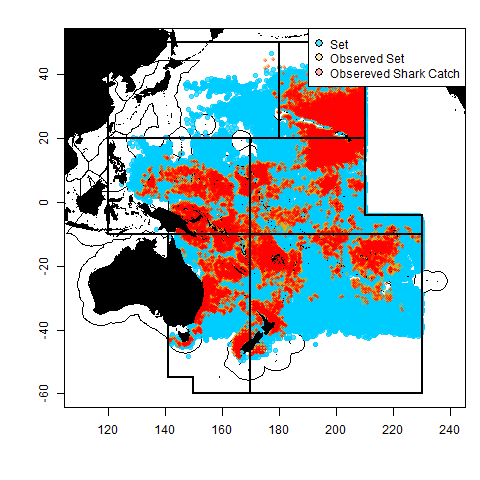
\includegraphics[scale=0.95]{../GRAPHICS/Defined/FIG_02_MAP_sets}
\caption{\label{fig:fig02} Map of WCPO and observed effort.}
\end{center}
\end{figure}

\begin{figure}
\begin{center}
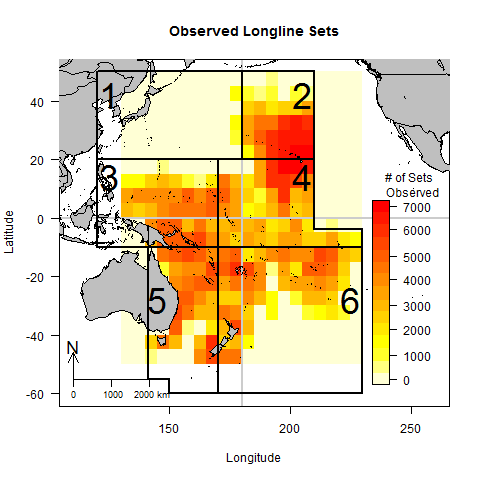
\includegraphics[scale=0.95]{../GRAPHICS/Defined/FIG_03_obs_ll_sets}
\caption{\label{fig:fig03} Longline observed sets by 5\degree x 5\degree square}
\end{center}
\end{figure}

\begin{landscape}
\begin{figure}
\centering
   \begin{subfigure}[b]{0.6\textwidth}
       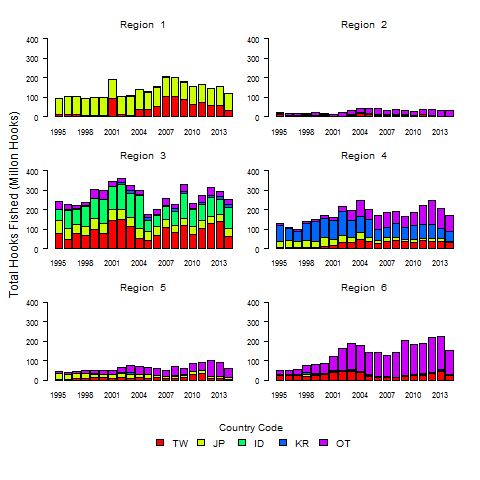
\includegraphics[width=\textwidth]{../GRAPHICS/Defined/FIG_04a_LLeff_FLAG_RDS}
       \caption{Longline effort.}
       \label{fig:test1}
   \end{subfigure}
   \begin{subfigure}[b]{0.6\textwidth}
       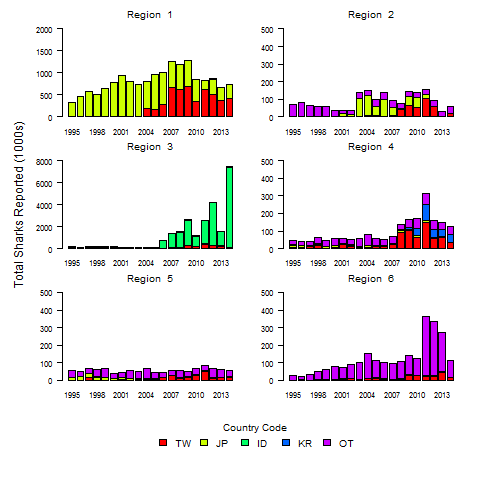
\includegraphics[width=\textwidth]{../GRAPHICS/Defined/FIG_04b_LLreported_catch_FLAG_RDS}
       \caption{Reported total shark catch.}
       \label{fig:test2}
   \end{subfigure}
\caption{Longline effort by flag and the number of sharks reported in logsheets}
\label{fig:fig04} 
\end{figure}
\end{landscape}

% FIGURE 5
\begin{landscape}
\begin{figure}
\centering
   \begin{subfigure}[b]{0.6\textwidth}
       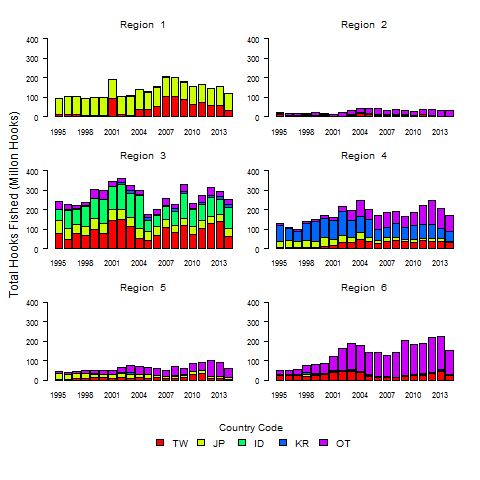
\includegraphics[width=\textwidth]{../GRAPHICS/Defined/FIG_05a_LLeff_FLAG_RDS}
       \caption{Longline effort.}
       \label{fig:test1}
   \end{subfigure}
   \begin{subfigure}[b]{0.6\textwidth}
       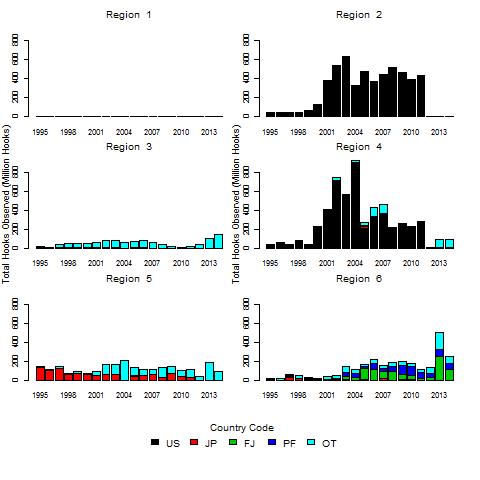
\includegraphics[width=\textwidth]{../GRAPHICS/Defined/FIG_05b_LLeff_obs_FLAG}
       \caption{Observer coverage.}
       \label{fig:test2}
   \end{subfigure}
\caption{Longline effort by flag and the extent of observer coverage}
\label{fig:fig05} 
\end{figure}
\end{landscape}

% FIGURE 6
\begin{landscape}
\begin{figure}
\centering
   \begin{subfigure}[b]{0.6\textwidth}
       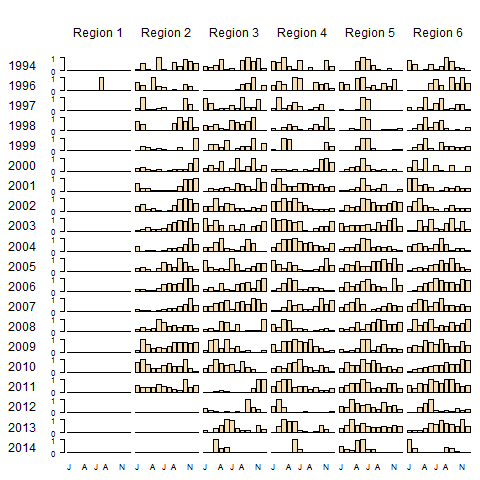
\includegraphics[width=\textwidth]{../GRAPHICS/Defined/FIG_06a_obsBY_mm_RDS}
       \caption{Longline effort.}
       \label{fig:test1}
   \end{subfigure}
   \begin{subfigure}[b]{0.6\textwidth}
       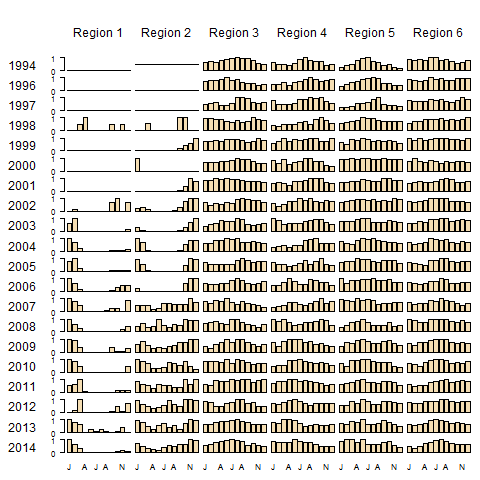
\includegraphics[width=\textwidth]{../GRAPHICS/Defined/FIG_06b_LOGSHEET_mm_RDS}
       \caption{Observer coverage.}
       \label{fig:test2}
   \end{subfigure}
\caption{Monthly breakdown of longline effort by region and the extent of observer coverage}
\label{fig:fig06} 
\end{figure}
\end{landscape}

%\addcenterfig[Logsheet effort by month.]{fig:logeffmnth}{}
%\addcenterfig[Observed effort by month.]{fig:obseffmnth}{FIG_xx_obsBY_mm}
%\addcenterfig[Absolute percent difference in effort between reported (logsheet)  effort and observed effort.]{fig:effdiff}{FIG_xx_obsDIFFlog_mm}

\clearpage
%\addcenterfig[Aggregate effort by region. ]{fig:aggeff}{FIG_xx_agg_eff}
 
%-------------------------------------------------------------------------------------------------------------------------
 
 \subsection{Purse Seine data} 
 %N.B. all the stats quoted here are in PS_oper_stats.r (JR)
Similar to the longline fishery, SPC-OFP holds logsheet data on shark catches by purse seine fisheries at both the operational and aggregate levels.  However, operational-level coverage for the purse seine fishery (87\%) is considerably higher than for the longline fishery (23\%). This factor, in combination with the more limited geographic range of the purse seine fishery, contributes to more representative operation-level coverage in the purse seine fishery than in the longline fishery.

Following implementation of the WCPFC ROP on 1 January 2010, in combination with prior observer coverage commitments by Parties to the Nauru agreement (PNA) members, 100\% purse seine observer coverage is now required (except for vessels fishing exclusively in one Exclusive Economic Zone (EEZ)). Historical observer coverage in the purse seine fishery has varied between EEZs. Coverage rates were low, generally less than 10\%, for the years 1995-2002, with coverage increasing to 10-18\% for the years 2003-2009. Recent (2010-2013) annual averages are between 42-56\% in total.


While observer coverage of the purse seine fishery is not uniformly representative (Figure \ref{fig:fig07}, orange points), it is more representative than observer coverage of the longline fishery, owing to both higher coverage levels and the more limited geographic range of the fishery (Lawson 2011). Regions 3 and 4 contain 98\% of the operational-level reported purse seine sets, and 99\% of observed sets and are thus the only regions for which purse seine analyses will be meaningful. Shark interactions are recorded in just 2.5\% of purse-seine operational logsheets (Figure \ref{fig:fig07}, red points), a value far lower than the 41\% recorded in longline operational-level logsheet. As a result, it is not possible to assess the number of shark interactions by set or the species involved using purse seine logsheet data.

A comparison by flag of purse seine effort and the number of purse seine sets reporting at least one shark interaction was constructed for associated (floating object) and unassociated (free-swimming) sets based on aggregated logsheet data (Figure \ref{fig:fig08}).  For each panel, flags were ranked by number of sets and the top four flags were plotted separately with all remaining flags aggregated into an "Other" category. Although estimated shark catches in the purse seine fishery are considerably lower than shark catches in the longline fishery (SPC 2008, Lawson 2011), it would still be expected that purse seine shark interactions are proportional to purse seine effort. However, from the discrepancies observed between the left and right panels, it appears that some major fishing nations are not submitting or are under-reporting their shark interactions.


%Figure 7
\begin{figure}
\begin{center}
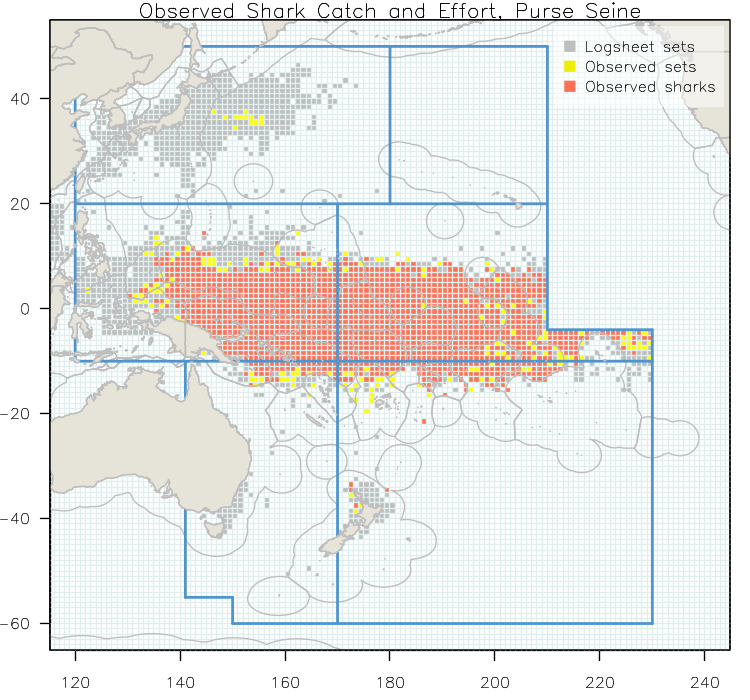
\includegraphics[scale=0.75]{../GRAPHICS/Defined/FIG_07_PS_sets}
\caption{\label{fig:fig07} Absolute percent difference in effort between reported (logsheet)  effort and observed effort.}
\end{center}
\end{figure}

% FIGURE 8
\begin{landscape}
\begin{figure}
\centering
   \begin{subfigure}[b]{0.49\textwidth}
       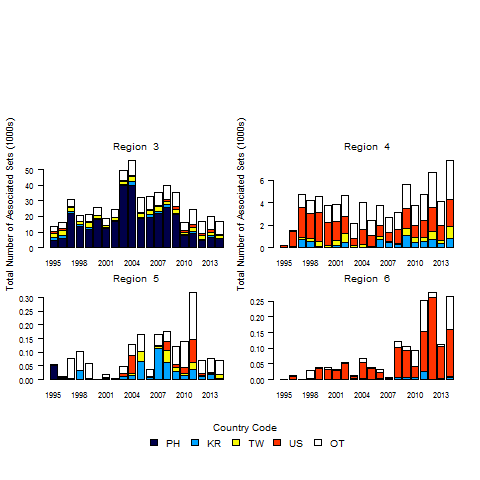
\includegraphics[width=\textwidth]{../GRAPHICS/Defined/FIG_08a_ps_total_effAssociated}
       \caption{Longline effort.}
       \label{fig:test1}
   \end{subfigure}
   \begin{subfigure}[b]{0.49\textwidth}
       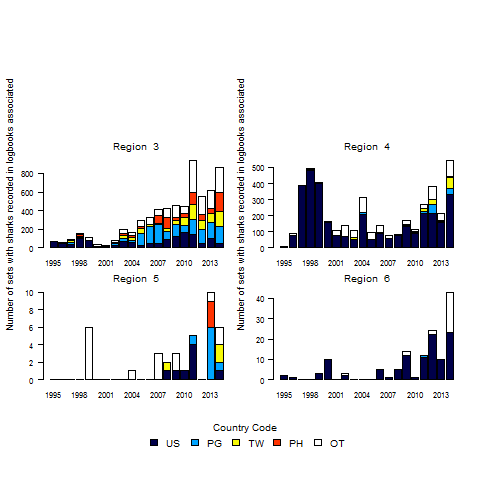
\includegraphics[width=\textwidth]{../GRAPHICS/Defined/FIG_08b_ps_oper_shks_rep_cntry_associated}
       \caption{Observer coverage.}
       \label{fig:test2}
   \end{subfigure}

   \begin{subfigure}[b]{0.49\textwidth}
       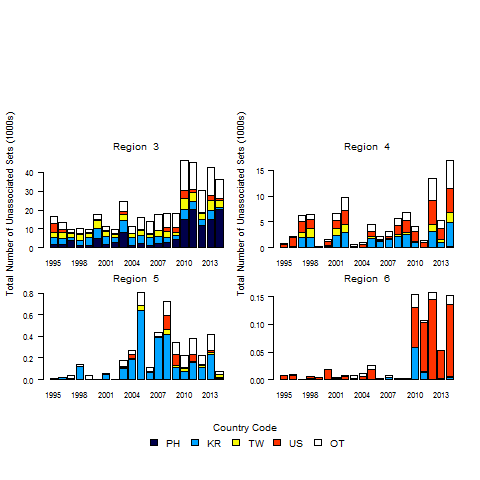
\includegraphics[width=\textwidth]{../GRAPHICS/Defined/FIG_08c_ps_total_effUnassociated}
       \caption{Longline effort.}
       \label{fig:test1}
   \end{subfigure}
   \begin{subfigure}[b]{0.49\textwidth}
       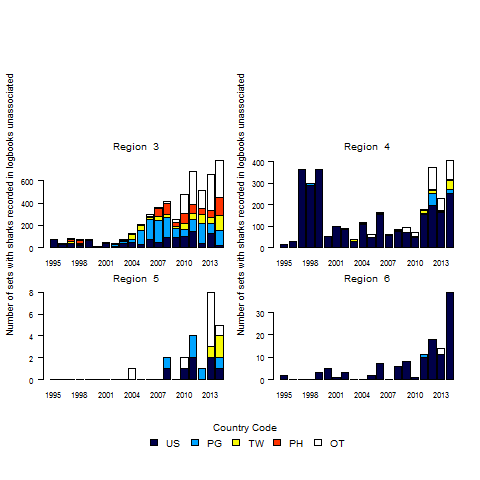
\includegraphics[width=\textwidth]{../GRAPHICS/Defined/FIG_08d_ps_oper_shks_rep_cntry_unassociated}
       \caption{Observer coverage.}
       \label{fig:test2}
   \end{subfigure}
\caption{Longline effort by flag and the extent of observer coverage}
\label{fig:fig08} 
\end{figure}
\end{landscape}

%  \addcenterfig[Absolute percent difference in effort between reported (logsheet)  effort and observed effort.]{fig:seine_map}{FIG_07_PS_sets}
 
 % old JR version 
 \begin{comment}
\hl{ As for the longline fishery, SPC-OFP holds logsheet data on shark catches by purse seine fisheries at the operational and aggregate levels, but operational-level coverage for the purse seine fishery,}
(87\%)  is considerably higher than for the longline fishery (23\%)
% sum(as.numeric( shklog$hook))/ sum(aggr$hhooks *100)
% print(paste0( "the operational level coverage of LL is ", round( 100* sum(as.numeric( shklog$hook))/ sum(aggr$hhooks *100),2   )))
% #"the operational level coverage of LL is 23.69"

This factor, in combination with the more limited geographic range of the purse seine fishery, contributes to more representative operation-level coverage in the purse seine fishery( \ref{fig:seine_map}  ) than in the longline fishery.

%\addcenterfig[Observed purse seine in the  WCPO showing the top four fishing nations and all others combined.  ]{fig:pssets}{FIG_xx_PS_eMAP_sets}


With implementation of the WCPFC ROP on 1 January 2010, in combination with prior observer coverage commitments by Parties to the Nauru Agreement (PNA) members, 100\% purse seine observer coverage is now required (except for vessels fishing exclusively in one exclusive economic zone (EEZ). Historical observer coverage in the purse seine fishery has varied between EEZs. Coverage rates were low, generally less than 10\% , for the years 1995-2002, with coverage incresing to 10-18\% for the years 2003-2009.  Recent  (2010-2013) annual averages are between 42-56\% in total. \hl{Although observer coverage of the purse seine fishery is not perfectly representative (Figure 2, orange points), the higher coverage levels and the more limited geographic range of the fishery result in more representative observer coverage for purse seines than for longlines (Lawson 2011 (Appendix Figure A2)). Regions 3 and 4 contain 98\% of the operational-level reported purse seine sets, and 99\% of observed sets and are thus the only regions for which purse seine analyses will be meaningful. In contrast to the longline operational-level logsheet data in which 41\% of recorded sets reported at least one shark}, only 2.5\% 
of purse seine operational-level logsheet sets reported any shark interactions (Figure \ref{fig:seine_map}, blue points). Due to inconsistent recording practices it is not possible to assess the number of shark interactions by set or the species involved using purse seine logsheet data.  

\hl{A comparison by flag of purse seine effort and the number of purse seine sets reporting at least one shark interaction was constructed for associated (floating object) and unassociated (free-swimming) sets based on aggregated logsheet data }
%Figure~\ref{fig:log_una_shk} \& Figure~\ref{fig:log_ass_shk}.

% note can we put the effort side by side with the shark reporting?
%  \addcenterfig[Comparison by region and flag of purse seine effort (in sets) associated sets using aggregated (5x5 degree square) data for six regions of the WCPFC Statistical Area, excluding data from Indonesia, Vietnam, and Japan coastal waters.]{fig:ps_ass_eff}{ps_total_effAssociated}
%   \addcenterfig[Comparison by region and flag of purse seine effort (in sets) unassociated sets using aggregated (5x5 degree square) data for six regions of the WCPFC Statistical Area, excluding data from Indonesia, Vietnam, and Japan coastal waters.]{fig:ps_una_eff}{ps_total_effUnassociated} 

%  \addcenterfig[Total sharks recorded on logsheets (in number of sets recording at least one shark interaction), for associated sets.]{fig:log_ass_shk}{ps_oper_shks_rep_cntry_associated}
%  \addcenterfig[Total sharks recorded on logsheets (in number of sets recording at least one shark interaction), for unassociated sets.]{fig:log_una_shk}{ps_oper_shks_rep_cntry_unassociated} 

For each panel, flags were ranked by number of sets and the top four flags were plotted separately with all remaining flags aggregated into an "Other" category.
Although estimated shark catches in the purse seine fishery are considerably lower than shark catches in the longline fishery (SPC 2008, Lawson 2011), it would still be expected that purse seine shark interactions are proportional to purse seine effort. However, from the discrepancies observed between the left and right panels in 
%Figure~\ref{fig:log_una_shk}
, it appears that some major fishing nations are not submitting or are under-reporting their shark interactions.
\end{comment} 
\clearpage         
 %       \subsection{Data formatting}
 %       \subsection{Limitations - Caveats}
        
        
%----------------------------------------------------------------------------------------
%  Distribuion Indicators
%----------------------------------------------------------------------------------------
             
        
\section{Distribution Indicator Analyses}
      \subsection{Introduction}

      Distribution indicators consider patterns in the geographic distribution of species catch. Spatial trends in fisheries data need to be interpreted carefully since they originate from a biased sampling design \citep{Walters2003_a}. If assessed carefully, however, they can provide useful insight into spatial and temporal trends in species distribution as well as highlight areas of strong interactions between a species and fisheries. In addition, changes in stock abundance might be reflected in distribution \citep{MacCall1990}, with increases and decreases in abundance resulting in range expansions and contractions, respectively. Such patterns have been reviewed at length in the terrestrial literature \citep{Borregaard2010_a} but less often for marine applications due to the paucity of historical data \citep[but see][]{Worm2011_a}. The indicators presented below are based on observer data and thus patterns in fishing effort and/or observer coverage may bias the results.  These results should therefore be interpreted as potential indicative of the location and intensity of interactions between these species and WCPO longline fisheries.  These indicators can be updated over time to determine if the spatial patterns change or temporal trends change.  More complex methodologies might also be applied to remove potential sampling biases.
      
\hllb{Potentially need to add back some of these.}\hl{These indicators examine the geographic range of each species and the habitat usage (in terms of geography only; oceanographic variables are not considered) by different life stages (adult/juvenile) and sexes based on fishery interaction data. Spatial analysis of fish occurrences can be useful in identifying range contractions or expansions which may be linked to fishing activities (Worm and Tittensor 2011). In addition, since many pelagic shark species are known to exhibit sex- and age- specific distribution patterns (Camhi et al. 2008, Mucientes et al. 2009) spatial analysis can highlight areas which are important to key life stages (e.g. presence of adult females and juveniles may indicate pupping grounds; presence of juveniles only may indicate nursery grounds).}
      
      
      \subsection{Methods}
      In this study, we calculated four Distribution Indicators:
      
\begin{itemize}
\item	Species-occurrence.  This indicator summarizes the occurrence of a species in any longline set monitored by an observer.  A positive value at any given location simply indicates that the species in question was observed at least once, without regard to annual frequency or fishing effort.

\item	Proportion-presence.  This indicator provides a rough indicator of the frequency of occurrence of each shark species in each region and trends in presence over time.  Using observer data, the indicator is computed by dividing the total number of sets with at least one occurrence by the total number of sets in each region/year combination.
\item	High-CPUE.  This indicator is intended to illustrate which regions and years have shown relatively high CPUE values for the different species.  The index is constructed, again on the basis of observed longline sets, by computing mean CPUE within each 5\degree $\times$ 5\degree cell within each of the six regions, and then calculating the proportion of cells within a region that are above a specific threshold.  For this analysis, the threshold was set at 1 shark per 1000 hooks for blue shark and at 1 shark per 5000 hooks for the other species.
\item	Catch-Hotspot.  This indicator is an extension of the Species-occurrence and Proportion-presence indicators, and is intended to illustrate the possible presence of variable species catch hotspots.  All observed data sets are totalled within 1\degree $\times$ 1\degree cells over four separate five-year (pentad) periods.  The proportion of observed sets containing at least one species occurrence within that cell/pentad cell is then computed and mapped.  This Catch-Hotspot indicator provides better temporal resolution than the Species-occurrence indicator and better spatial resolution than the Proportion-presence indicator in helping to identify the distributional patterns of each shark species.
\end{itemize}



      \subsection{Results}
      
      The four sets of Distribution Indicators are grouped in Appendix A, as follows: Species occurrence (Figures \ref{IA_01} to \ref{IA_07}), Proportion-presence (Figure \ref{IA_08}), High-CPUE (Figure \ref{IA_09}), Hot spot analysis (Figures \ref{IA_10} to \ref{IA_16}).  Species-specific results below reference these sets of figures.
      
        \subsubsection{Blue Shark}
Blue sharks are the most common and widely reported shark bycatch species in the WCPO longline fisheries.  They are found to occur through the range of longline fishing and have the highest proportion-presence rate in virtually all years and regions among the shark species analysed in this report.  Both the Proportion-presence and High-CPUE time series show distinct downwards trends from the late 1990s to the present in most regions (3, 5, and 6).  The Catch-hotspot indicator shows consistently high occurrence of blue shark in longline fishery around the Hawaiian Islands with occurrence generally declining to the south, before again increasing in frequency around 20\degree{}S.




%\addcenterfig[Blue shark distribution indicators. Proportion of positive sets, observer data.]{fig:bsh1}{FIG_xx_pcntpos_reg_BSH}
%\addcenterfig[Blue shark distribution indicators. Proportion of 5 degree squares having CPUE greater than 1 per 1000 hooks region, observer data.]{fig:bsh2}{FIG_xx_HIGH_CPUE_BSH}
%\addcenterfig[Blue shark distribution indicators. Life stage and sex distribution.]{fig:bsh3}{Map_maturity_sex_BSH}

%----------------------------------------------------------------------------------------
\subsubsection{Mako Shark}
Mako sharks are one of the most commonly captured shark species in the longline fisheries of the WCPO.  Mako sharks have been encountered in longline sets in all regions that observers have sampled.  The largest, most consistent, hotspots have included waters in Region 5 between Australia and New Zealand.  Spatially, there are differing trends over time in the Proportion-presence and High-CPUE indicators.  The north and west regions (2 and 3) show stable or slightly increasing rates (though data for region 2 is lacking for years 2012-2014) whereas the south Regions (5 and 6) show steadily declining rates.

%\addcenterfig[Mako shark distribution indicators. Proportion of positive sets, observer data.]{fig:mak1}{FIG_xx_pcntpos_reg_MAK}          
%\addcenterfig[Mako shark distribution indicators. Proportion of 5 degree squares having CPUE greater than 1 per 1000 hooks region, observer data.]{fig:mak2}{FIG_xx_HIGH_CPUE_MAK}
 %\addcenterfig[Mako shark distribution indicators. Life stage and sex distribution.]{fig:mak3}{Map_maturity_sex_MAK}         
          
%----------------------------------------------------------------------------------------
 \subsubsection{Silky Shark}
 Silky sharks are commonly encountered in Regions 3 through 6 and at a very low rate in Region 2.  Neither the Proportion-presence nor High-CPUE indicators illustrate sustained temporal trends in occurrence.  The region with the greatest proportion of High-CPUE occurrence is Region 3.  The Catch Hotspot indicator also illustrates a consistency in both the temporal and spatial encounter of the LL fishery with silky sharks.
 %JR: For silky shark there seems to be a slight downward trend in the core regions of 3 and 4
%\addcenterfig[Mako shark distribution indicators. Proportion of positive sets, observer data.]{fig:fal1}{FIG_xx_pcntpos_reg_FAL}           
%\addcenterfig[Silky shark distribution indicators. Proportion of 5 degree squares having CPUE greater than 1 per 1000 hooks region, observer data.]{fig:fal2}{FIG_xx_HIGH_CPUE_FAL}
%\addcenterfig[Silky shark distribution indicators. Life stage and sex distribution.]{fig:fal3}{Map_maturity_sex_FAL}
%----------------------------------------------------------------------------------------
 \subsubsection{Oceanic Whitetip Shark}
 Oceanic whitetip sharks also occur with regular frequency in observed longline sets through most of the WCPO longline fisheries.  In the five regions where they are commonly encountered (Region 1 contains few observed sets) the trend in both Proportion-presence and High-CPUE has been steadily downward since the mid-1990s, with some of the decline in rates exceeding 80\%.  Catch-hotspots for oceanic whitetip sharks have been in the central Pacific, particular the region surrounding the junction of Regions 3, 4, 5, and 6.
 %\addcenterfig[Oceanic whitetip shark distribution indicators. Proportion of positive sets, observer data.]{fig:ocs1}{FIG_xx_pcntpos_reg_OCS}          
 %\addcenterfig[Oceanic whitetip shark distribution indicators. Proportion of 5 degree squares having CPUE greater than 1 per 1000 hooks region, observer data.]{fig:ocs2}{FIG_xx_HIGH_CPUE_OCS}
 %\addcenterfig[OCeanic whitetip shark distribution indicators. Life stage and sex distribution.]{fig:ocs3}{Map_maturity_sex_OCS}         

%----------------------------------------------------------------------------------------
 \subsubsection{Thresher Shark}
 Thresher sharks have been found in observed longline sets in most regions of the WCPO with the possible exception of the area around French Polynesia. Catch-hotspots have been north of the equator, especially in Region 4. Both the Proportion-presence and High-CPUE time series show indistinct temporal trends though Regions 3 and 4 have dropped considerably over the past five years.
%in recent years an increase in the proportion of positive sets was evident.
%\addcenterfig[Thresher shark distribution indicators. Proportion of positive sets, observer data.]{fig:thr1}{FIG_xx_pcntpos_reg_THR} 
%\addcenterfig[Thresher shark distribution indicators. Proportion of 5 degree squares having CPUE greater than 1 per 1000 hooks region, observer data.]{fig:thr2}{FIG_xx_HIGH_CPUE_THR}
  %\addcenterfig[Thresher shark distribution indicators. Life stage and sex distribution.]{fig:thr3}{Map_maturity_sex_THR}         

%----------------------------------------------------------------------------------------
 \subsubsection{Hammerhead Shark}
 Among the shark species analysed in this report, hammerhead sharks have the lowest encounter rates (measured as Proportion-presence) and appear to be patchily distributed.  The regions with the apparent largest presence of hammerhead sharks is the Northeast (Hawaiian Islands) and Southwest (Papua New Guinea, Australia east coast).  Due to the low encounter rates, little inference can be made regarding temporal trends in occurrence.
 
%\addcenterfig[Hammerhead shark distribution indicators. Proportion of positive sets, observer data.]{fig:hhd1}{FIG_xx_pcntpos_reg_HHD} 
%\addcenterfig[Hammerhead shark distribution indicators. Proportion of 5 degree squares having CPUE greater than 1 per 1000 hooks region, observer data.]{fig:hhd2}{FIG_xx_HIGH_CPUE_HHD}
  %\addcenterfig[Hammerhead shark distribution indicators. Life stage and sex distribution.]{fig:hhd3}{Map_maturity_sex_HHD}         
         
%----------------------------------------------------------------------------------------
 \subsubsection{Porbeagle Shark}
 Porbeagle sharks have historically only been encountered in the southern region of the WCPO, essentially only south of 20 \degree S (Regions 5 and 6).  A decrease in the spatial and temporal occurrence of porbeagle in observed sets is evident in the three Distribution Indicators other than Species-occurrence.  The porbeagle catch-hotspots have shrunk both in size and intensity over the four pentads; the Proportion-presence and High-CPUE time series for Regions 5 and 6 have declined as much as 90\% over the past 15 years.
 
%JR: Porbeagle sharks in region 5 and 6 show slightly increasing to stable trends. 

%\addcenterfig[Porbeagle shark distribution indicators. Proportion of positive sets, observer data.]{fig:por1}{FIG_xx_pcntpos_reg_POR} 
%\addcenterfig[Porbeagle shark distribution indicators. Proportion of 5 degree squares having CPUE greater than 1 per 1000 hooks region, observer data.]{fig:por2}{FIG_xx_HIGH_CPUE_POR}
  %\addcenterfig[Porbeagle shark distribution indicators. Life stage and sex distribution.]{fig:por3}{Map_maturity_sex_POR}         
         





      \begin{comment}
      \hl{The following points were noted from the life stage and sex distribution plots:
- Adult blue sharks were more common than juveniles in the waters off Hawaii and at latitudes of 20$^{\circ}$S this corresponds to the blue shark mating ground proposed by Nakano (1994); 

- The observed distributions of adult and juvenile oceanic whitetip and silky sharks are similar but samples of silky sharks were particularly skewed toward juveniles in tropical waters.
- Thresher sample sizes were small but were mainly comprised of juveniles in tropical areas.}
- Observer records of hammerhead sharks that include sex and length were extremely limited, the samples were proportionally more juvenilles in the tropical waters around Paupa New Guinea and Fiji.
-Oservations of porbeagle sharks are  limited to mid-year samples in the waters around Tasmania, where they tend to higher proportions of adults.
\end{comment}

\clearpage         
%----------------------------------------------------------------------------------------
        
     
          
  \subsection{Conclusions}
  
\hllb{With the exception of blue shark the high-CPUE indicator more or less steady trends for all species in all regions, however this analysis was hampered by the lack of data throughout the region for species.} %JR
  
Intrepretation of the   distribution indicators is complicated by the influence of changes in fishing effort,  potential  changes in community composition, obsservational coverage  and operational factors influencing selectivity and catchability (e.g. depth and leader material). As such, these indicators are best used for identifying the areas in which species-fishery interactions take place, and as supporting information for interpreting other patterns and trends. 
% Distribuion Indicators 




%----------------------------------------------------------------------------------------
%  Species Composition
%----------------------------------------------------------------------------------------
      
      
\section{Observed Species Composition Indicator Analyses}

 \subsection{Introduction}
\hl{The species composition of the catch, as recorded by longline and purse seine observers, was examined to identify any apparent changes over time. This type of analysis reinforces the species-specific fishery interaction information above, but supplies more detail on interactions by separating longline sets by depth and purse seine sets by type of school association. Another important reason for examining catch composition indicators is to assess changes in the percentage of unidentified shark species over time. Improvements in the observers' ability to identify sharks could contribute to increasing occurrences of species-specific records in the observer database and could bias temporal trends.}

\hl{While this analysis provides information on the relative proportions of the key species within the observer samples, estimation of total catch composition and quantity is complicated by issues of observer sample coverage and representativeness (see Section 2) and is the subject of a separate analysis (Lawson 2011). Regardless of whether catch composition indicators are based on observer samples or the entire catch, changes in species composition over time can suggest relative population increases or depletions. However, species-specific catch rate analyses should be performed to directly assess whether actual abundances for individual species have changed (see Section 5).}
     
%      \subsection{Methods}
%      \subsection{Results}
      
  \subsubsection*{Longline}  
  

With just a few exceptions, blue shark catch dominates the longline shark bycatch.  In Regions 2, 4, 5, and 6, blue sharks have average 60-90\% of shark bycatch; in Region 4 the proportion of blue shark has dropped from around 60\% in the late 1990s to 10-15 in recent years.  The second most common observation of shark species, in terms of numbers, is silky shark which have constituted a majority of shark bycatch in Region 3 since the early 2000s and have been on the order of 5-10\% in \ other regions.  We note that there appears to be a sudden increase in the proportion of silky shark catch for Region 4 in years 2012-2104.  In fact, this reflects the absence of observer data from the U.S. longline fleet operating around Hawaii which constituted the large majority of longline sets in that region dating back to the start of the time series.  As evidenced by the small number of observed sets shown for years 2012-2014, the shark composition data for these years in Region 4 are quite likely very unrepresentative.  Several of the other shark species constitute up to 10\% of the shark bycatch in certain regions and time periods: porbeagle in Regions 5 and 6, oceanic white tip sharks in Regions 3, 4, and 6 and thresher sharks in regions 3 and 4.  The \hl{estimated proportion} of unidentified sharks is quite low in all regions, which may reflect indicate that the   composition of shark bycatch in tuna fisheries is composed of the mostly the species listed as key shark species.  

Division of the longline shark bycatch into shallow and deep sets revealed several differences in the assemblage of sharks caught at depth.  Regions 3, 5, and 6 each have relatively large number of observed sets (Regions 1, 2 and 4 have essentially no observed sets in one or the other depth characterization) so we restrict our comparison to those Regions.  In the southern Regions (5 and 6), blue shark and porbeagle comprise as much as 95\% of the longline shark catch; the deep water sets contain a much more diverse array of species with silky, thresher, oceanic whitetip and mako sharks occurring in substantial numbers.  Differences in shark composition in Region 3 are much more subtle than Regions 5 and 6; hammerhead and oceanic white tip sharks are more common in deep sets while silky sharks are a bit more common in shallow sets.


\begin{comment}  
 \hl{ As expected, blue sharks dominated the shark records from the longline fishery, comprising on average 69-91\% of the observed catch in Regions 2, 4, 5 and 6 for 1995-2014 (Figure 14, top panel). In Region 3 silky sharks were the most frequently encountered sharks comprising 64\% of the observed catch in 1995-2014. Small numbers of mako and oceanic whitetip sharks were recorded in temperate and tropical areas respectively. Thresher sharks, predominantly bigeye threshers, comprised on average 12\% of the observed catch in Region 4 but were rarely recorded in other regions. The non-key species observed in Regions 5 and 6 were primarily composed of porbeagles, roughskin dogfish (Centroscymnus owstoni) and tope shark (Galeorhinus galeus), and in Region 3 were primarily composed of unidentified hammerhead, grey reef (Carcharhinus amblyrhynchos) and blacktip (Carcharhinus limbatus) sharks. Unidentified sharks comprised no more than 1.6\% of the recorded sharks in any of the regions.}
  
 \hl{ Species composition is plotted by set depth in the lower panel of Figure 8, using hooks per basket as a proxy variable to separate shallow ($<$11 hooks per basket) from deep sets ($>=$11 hooks per basket). This comparison illustrates that although there were more deep sets conducted in Region 3 than shallow sets (n=3,318 versus n=2,181), most of the silky sharks in Region 3 are caught in the shallow sets. The vast majority of sets in Regions 4 and 6 were deep sets and it is these sets which produced the catches of blue and thresher sharks. Shifts in Regions 2 and 5 from shallow to deep sets may reflect changes in fishery regulations in Australia (AFMA 2008) and the US (Walsh et al. 2009), but both types of sets catch primarily blue sharks. }
 
\end{comment}

  
%------------------------------------------------------------------------------------------
 \subsubsection*{Purse Seine} 
 
\hl{ Plots of the catch composition as recorded by observers in the purse seine fishery indicate that unlike for longlines, a non-negligible portion of the sharks recorded in the first half of the time series (1995-2003) were not identified to species (i.e. UID; Figure 9). As discussed in Section 2, this is probably a function of the practical difficulties in recording purse seine-caught sharks which are not hauled onboard, but the problem appears to have been resolved in recent years. Overall, approximately 70\% of the observer-recorded catch was silky shark; the next most abundant species was oceanic whitetip shark which comprised 7\% of the records. The numbers of sets shown in the lower panels illustrate that associated sets comprised 67\% of the observer samples in Region 3 and 59\% of the samples in Region 4, but recorded 88\% and 93\% of the sharks respectively. It is also noted that oceanic whitetip sharks were observed in substantial numbers only in associated sets and only until 2004-2005.}
 
 \subsection{Conclusions}

The Species Composition indicators reveal that shark bycatch differs substantially between longline and purse seine fishing in the WCPO.  

Blue sharks are the most prevalent longline caught shark, but there are substantial regional and depth variations.  Several species are commonly caught more frequently in deeper sets; porbeagle form a sizable component of the shallow sets in Regions 5 and 6 and silky shark is the second most common longline caught shark.

Purse seine shark bycatch is much less variable and is dominated by silky sharks, particularly over the past decade when the number of observed sets increased greatly and composition data may have become more representative.  In virtually all regions and years, silky shark comprises more than 95\% of the shark bycatch, with minor numbers of hammerhead and oceanic whitetip sharks occurring.  Oceanic white tip sharks appear to have been more common prior to 2000, their percentage contribution to the overall shark cath has not been more than 20\% in regions 3 and 4 for over a decade, which is stark contrast to the first ten years of the study period. 

 
\hl{ The observed longline catch composition plots illustrate that blue shark dominate in most regions. An exception to this pattern is Region 3 where silky sharks, primarily from shallow sets, are the most frequently observed species. Although there are some minor differences in species composition between observed shallow and deep sets in other regions (e.g. Regions 2 and 4), these may be related to sampling representativeness. Analysis of observed purse seine shark catches reveals that silky sharks predominate with the majority of these found in associated sets. In previous years, oceanic whitetip shark was the second-most commonly identified shark in associated sets but this species has been only rarely observed in recent years. Substantial numbers of sharks caught by purse seines were unidentified until 2002-2003.}
      
 \clearpage          

%----------------------------------------------------------------------------------------
%  CPUE INDICATORS
%----------------------------------------------------------------------------------------
\section{Catch Per Unit Effort indicator analyses}

%\documentclass{SCreport}

%\begin{document}
%%%%%%%%% Defining latex macros to print tables %%%%%%%%%%


\newcommand{\blueaic}{
% latex table generated in R 3.2.0 by xtable 1.7-4 package
% Sat Jul 04 14:52:03 2015
\begin{table}[ht]
\centering
\caption{AIC improvement over null model for blue from a single explanatory variable} 
\label{blue:aic1}
\begin{tabular}{lrr}
  \hline
Variable & AIC.diff & AIC.diff.sigma \\ 
  \hline
program\_code & 24382.47 & 16607.68 \\ 
  flag\_id & 23711.29 & 17163.94 \\ 
  HPBCAT2 & 20183.28 & 5765.59 \\ 
  HPBCAT & 20178.74 & 5576.42 \\ 
  yy & 14357.75 & 8612.54 \\ 
  mm & 3725.06 & 2511.55 \\ 
  sharkbait & 994.97 & 454.07 \\ 
   \hline
\end{tabular}
\end{table}

}


\newcommand{\makonorthaic}{
% latex table generated in R 3.2.0 by xtable 1.7-4 package
% Sat Jul 04 14:52:03 2015
\begin{table}[ht]
\centering
\caption{AIC improvement over null model for mako.north from a single explanatory variable} 
\label{mako.north:aic1}
\begin{tabular}{lrr}
  \hline
Variable & AIC.diff & AIC.diff.sigma \\ 
  \hline
HPBCAT2 & 6433.14 & 642.33 \\ 
  HPBCAT & 6417.24 & 640.61 \\ 
  mm & 2845.80 & 216.50 \\ 
  yy & 2216.05 & 401.91 \\ 
  flag\_id & 115.74 & 61.51 \\ 
  program\_code & 114.17 & 44.28 \\ 
  sharkbait & 15.46 & 3.29 \\ 
   \hline
\end{tabular}
\end{table}

}


\newcommand{\makosouthaic}{
% latex table generated in R 3.2.0 by xtable 1.7-4 package
% Sat Jul 04 14:52:03 2015
\begin{table}[ht]
\centering
\caption{AIC improvement over null model for mako.south from a single explanatory variable} 
\label{mako.south:aic1}
\begin{tabular}{lrl}
  \hline
Variable & AIC.diff & AIC.diff.sigma \\ 
  \hline
program\_code & 1693.97 & 251.6 \\ 
  flag\_id & 1438.39 & --- \\ 
  HPBCAT2 & 1202.23 & 79.45 \\ 
  HPBCAT & 1127.42 & 34.67 \\ 
  yy & 875.66 & 389.5 \\ 
  mm & 733.11 & 178.28 \\ 
  sharkbait & 8.37 & -1.89 \\ 
   \hline
\end{tabular}
\end{table}

}


\newcommand{\ocsaic}{
% latex table generated in R 3.2.0 by xtable 1.7-4 package
% Sat Jul 04 14:52:03 2015
\begin{table}[ht]
\centering
\caption{AIC improvement over null model for ocs from a single explanatory variable} 
\label{ocs:aic1}
\begin{tabular}{lrr}
  \hline
Variable & AIC.diff & AIC.diff.sigma \\ 
  \hline
yy & 3726.21 & 958.91 \\ 
  program\_code & 2781.62 & 1369.09 \\ 
  flag\_id & 1499.89 & 772.13 \\ 
  sharkbait & 887.50 & 103.91 \\ 
  HPBCAT2 & 308.22 & 1656.57 \\ 
  HPBCAT & 256.09 & 1658.57 \\ 
  mm & 143.92 & 185.56 \\ 
   \hline
\end{tabular}
\end{table}

}


\newcommand{\silkyaic}{
% latex table generated in R 3.2.0 by xtable 1.7-4 package
% Sat Jul 04 14:52:03 2015
\begin{table}[ht]
\centering
\caption{AIC improvement over null model for silky from a single explanatory variable} 
\label{silky:aic1}
\begin{tabular}{lrr}
  \hline
Variable & AIC.diff & AIC.diff.sigma \\ 
  \hline
program\_code & 10913.31 & 6886.75 \\ 
  flag\_id & 10144.24 & 5446.47 \\ 
  sharkbait & 5382.46 & 1713.24 \\ 
  yy & 4986.96 & 3273.31 \\ 
  HPBCAT2 & 1639.75 & 4527.65 \\ 
  HPBCAT & 1628.44 & 4513.75 \\ 
  mm & 957.50 & 358.96 \\ 
   \hline
\end{tabular}
\end{table}

}



\subsection{Introduction}

%This paper follows from the previous indicator based analysis presented to the Western and Central Pacific Fisheries Commission (WCPFC) Scientific Committee (SC7, Clarke et al. 2011), stock assements (Rice et al. 2014, Rice et al.2013, Rice et al.2012) \hllb{(cite the standardization papers, cite ISC work?)}. The developments presented here include additional analyses of the Secretariat of the Pacific (SPC) data holdings for silky caught in longline and purse seine fisheries in the Western and Central Pacific Ocean (WCPO), though we note that some previous data (Japan) was not available for this effort. Standardized catch per unit of effort (CPUE) series are developed for the main shark species.  
%\emph{Note: The current analysis does not construct inputs to use for stock assessments or catch estimates. Our goal is to highlight general trends in population abundance over time, to be interpreted together with other indicators as outlined above. We recommend that catch rates standardization for stock assessments or catch estimates be conducted independently.}


% intro      
Catch-per-unit-effort (CPUE) data are commonly used as indices of abundance for marine species. However, multiple factors---fishing technique, season, bait type, etc---can alter the relationship between CPUE and abundance, especially in complex fisheries systems comprising of several fleets and spanning large spatial and temporal scales. Nominal catch rates must therefore be standardized to account for changes in these factors over time. This is typically done using General Linear Models (GLM), which allow us to model the relationship between CPUE and a set of explanatory variables. The dataset used in this analysis provided many candidate variables, but, given the diversity of observer programs represented, few had enough coverage to be retained in the final models. The available variables are described in Table \ref{tbl:glm-vars} (see also Table 2 in \citet{Francis2014_b} for an overview of the use of variables in shark CPUE standardisations).

% issue with sharks cpue standrz
CPUE data for sharks often have a large proportion of observations (sets) with zero shark catch, while while some sets have large catch. These instances of high catch can occur when areas of high shark densities are accidentally encountered or when fishers target sharks. The co-existence of both high proportions of zeros and high catch results in over-dispersed data, typical of bycatch species. These features are challenging to account for from a statistical point of view, and have been reviewed at length in the literature on bycatch analyses \citep{Bigelow2002_a,Campbell2004_a,Ward2005_a,Minami2007_a}. 
%(Bigelow et al. 2002; Campbell 2004, Ward and Myers 2005; Minami et al. 2007).

Zero-inflated approaches have been advocated as best suited to model over-dispersion in both zeros and positive counts (Brodziak et al., 2013). A drawback of the zero inflated approach is that it is data intensive and models fail to converge. In addition, in practice it tends to be more successful at modelling the extra zeroes than the large-catch events, since the dispersion parameter which controls the length of the tail is assumed to be constant over all factors. This is especially a problem when the mean of the distribution is close to zero or one, as in those instances the probability of getting large events if mostly controlled by the dispersion parameter $\sigma$, unlike when the mean is larger and the tail is not as pronounced. However, whenever conditions are good for sharks and/or targeting takes place, larger catch events can happen and not modelling those properly implies that we are missing important drivers of catch. Typically, this can be diagnosed as a departure from the one-to-one line on the right-hand side of quantile-quantile plots. Here we achieved significant improvements in model diagnostics by keeping a negative binomial distribution but allowing both the mean $\mu$ and $\sigma$ parameters to be modelled against covariates \citep{Rigby2005_a}. This approach is much less computationally intensive than zero-inflated models, and yielded excellent diagnostics with these data.


 \subsection{Methods}
Standardised CPUE series for the longline bycatch fisheries were developed using generalised linear models using longline catch and effort data. The number of hooks in a longline set was used as a measure of effort.
See also \citet{Clarke2011_a, Clarke2011_b},  \citet{Walsh2011_a}, \citet{Rice2012_a}   for past work on shark CPUE standardisation in the Western and Central Pacific Ocean (WCPO).
%  @Article{,
 %   title = {Generalized additive models for location, scale and shape,(with discussion)},
 %   journal = {Applied Statistics},
 %   volume = {54},
 %   part = {3},
 %   pages = {507-554},
 %   year = {2005},
 %   author = {R. A. Rigby and D. M. Stasinopoulos},
 % }
 \label{cpuemeth:datafilter}
 \subsubsection{Stock definition for the purpose of the analysis}
   
% talk about stocks and year span                                                                                        
%Silky and oceanic white tip sharks are observed mainly in the equatorial waters in the purse seine fishery (Figure \ref{...}), and from about -25\degree~S to 25\degree~N in the longline fishery (Figure 1). 
Silky and oceanic whitetip sharks have each been assessed \citep{Rice2012_a, Rice2013_a} as single stocks in the WCPO, and are presented in this analysis as a single stock.  Thresher, mako and blue sharks occur more frequently in cold, temperate waters, and generally believed to be separated into northern and southern stocks. For instance, blue sharks in the North Pacific have been subject to multiple stock assessments as a stock unit. These temperate species are thus analysed as individual stocks. In the Pacific porbeagle sharks are only found south of 20\degree{}S and were analysed as a single stock. Hammerhead sharks for the purpose of this analysis (and throughout the report) are considered to be a single stock.

\subsubsection{Data Preparation}
To further define the expected geographic range, we defined a coarse climate `envelope' based on sea surface temperature. This aided in distinguishing between zero catch in areas where the species does not occur from zero catch in areas where the species occurs but was not caught. Temperature data were downloaded from the GODAS database (\url{www.cdc.noaa.gov/data/gridded/data.godas.html}) and matched to the observer data on a set by set basis. The temperature range of a species was defined as the minimum and maximum of the monthly mean sea surface temperatures (SST) of cells with positive catch for that species (see Table \ref{meth:temprange}). The temperature predicted by GODAS at the 5 meters depth at set time/day was used for the SST value. Only cells for which all mean monthly temperatures fell within this range were retained. %\hllb{REWORK. Note that this is a minimal filter and it was only used to exclude the most improbable cells from which a species could be seen.}
 %\hl{Looked at range of SST where positive catches occured, selected cells where median falls within this range.}
 
%                                                                        section \ref{app:datacleaning}     
          
Data were cleaned following the filters outlined in Table \ref{tbl:datfiltering}. Records from the US observer programs (Hawaii and American Samoa) were excluded from the analysis as they were only available up to 2011. Records from any observer programs for which we had less than 100 sets were removed. Extreme catch events greater than the $97.5^{th}$ quantile of the nominal CPUE were also removed. Finally, year effects were only estimated if there were at least 50 sets observed in that year (by species and population).  Records from the Papua New Guinea observer program were removed as vessels in the fleet frequently target sharks. Additional filters are listed by species in Table \ref{tbl:glmdata}.
                                                                                      
%Previous work \citep{Rice2012_a, Rice2013_a, Bromhead2012_a} has examined the extent of shark targeting in the WCPO tuna longline %fleet, and found that a number of factors (i.e. sharklines, wire trace can lead to a higher catch rates). Shark target sets comprise a much smaller proportion of the overall dataset (6.5\% of the sets), however, these sets represent significant shark catch for some species (e.g. 82\% of the total silky shark catch). Sets marked by observers as targeting sharks were therefore removed from the analysis as catch rates therein behave differently than when sharks are caught as by-catch. 
%Shark targeting sets were deemed to be sets where the observer had marked that the set was intentionally targeting sharks of any species, whether shark bait was used, or whether shark lines were used. We also removed the data from the Papua New Guinea observer program because of frequent shark targeting which may not always appear in observer records. 
                                                                                       
% \subsection{Additional categorical variables}    % jr edits don't think we need that
% 1. Day category: sunset and sunrise were calculated\\ 
% 2. HPBCAT: based on data exploration two types explored: either shallow or deep (with shallow $<=$ 10), or HPBCAT2 shallow, intermediate and deep, with intermediate between 10 and 15 ... in general hpbcat2 had slighlty better aic %(in tables at the end)
     %Latitude and longitude were truncated to the nearest 1\degree; this location information was used to calculate the set specific association with a 5\degree square (referred to hereinafter as cell). Date of set was used to calculate the year, month, quarter and trimester of the set. Set time was used to calculate the time category of the day in sixths starting at midnight. A non-target data set was created as a result of filtering data sets according to the above rules as well as filtering sets where sharks were the intentional target. This was done under the premise that the factors leading to non-zero catch rates when targeting sharks would be different than factors that lead to non-zero catch rates when not targeting sharks. 
                                                                                       
                                                                                       
   \subsection{Overview of GLM Analyses}
   \subsubsection{Notes on error distributions:} 
  
   The  filtered datasets  were standardised using generalized linear models \citep{McCullagh1989_a} with the software package R (\url{www.r-project.org}, \citealt{RCT2013_a}) and the package \texttt{gamlss} \citep{Rigby2005_a}. Initially, multiple assumed error structures were tested including the delta lognormal approach (DLN)   \cite{Lo1992_a, Dick2006_a, Stefansson1996_a}, zero-inflated poisson and negative binomial models, the tweedie distribution \citep{Shono2008_a} and negative binomial models with mu and  $\sigma$ modelled. Due to its superior performance both in run time and model diagnostics, we retained the latter and only present those results here.
%  in JR_bib_edts.bak Hiroshi Shono 2008. Application of the Tweedie distribution to zero-catch data in CPUE analysis. Fisheries Research 93 (2008) 154-162

%The negative binomial (Lawless, 1987) is typically more robust to issues of over-dispersion (over-dispersion can arise due to excess zeros, clustering of observations, or from correlations between observations) was also used. This model has been advocated as a model that is more robust to over-dispersion than the Poisson distribution (McCullagh and Nelder 1991), and is appropriate for count data (Ward and Myers  2005), but does not expressly relate covariates to the occurrence of excess zeros (Minami et al. 2007).
                                                                                       
 %    	Mixture models such the zero inflated Poisson (ZIP) and zero inflated negative binomial (ZINB) (Zuur 2009, Cunningham and Lindenmayer 2005, Welsh et al. 2000): these models are useful for modelling counts of rare species when the number of zero observations is larger than expected. Zero inflated models are a process similar to the delta approach in which the presence or absence of the catch is modelled orthogonally to the size of the catch (Welsh et al 2000), however unlike the delta approach the count data can include zeros. These zeros could result from predator satiation, competition for hooks, or disinterest (called true zeros) as opposed to design errors, sampling errors, observer errors or zeros resulting from sampling outside the habitat range (called false zeros). The total probability of a zero count is then,
\subsubsection{Procedure for model selection}
% cite AIC?Akaike, H. (1974), "A new look at the statistical model identification" (PDF), IEEE Transactions on Automatic Control 19 (6): 716-723, doi:10.1109/TAC.1974.1100705, MR 0423716.  get the table refs right 
Initial model exploration began via fitting each model (species and population) with only one covariate and evaluating the explanatory power of that covariate \via AIC (AIC values are listed in tables  listed in Tables~\ref{BSH.north:aic1} to \ref{THR:aic1}. Model fitting proceeded by fitting additional covariates in order of the proportion of deviance explained  on their own.  Only those covariates showing a change in AIC of 10 or greater were kept in the model.
%-- added covariate on MU ONLY (mean) until AIC showed decline $<$ 10 (arbitrary....) \\

If model diagnostics indicated a departure from the assumed error structure, covariates were added to $\sigma$ until the model mis-specification was resolved. Covariates were added based on the principle of a minimally efficient design and beginning with those covariates for which the AIC~$\sigma$ table (Tables \ref{BSH.north:aic1} to \ref{THR:aic1}) indicated had the most explanatory power.  

The addition of explicitly modelling the $\sigma$ greatly improved the  model diagnostics in  most cases where the Q-Q norm plot indicated a misspecification in the tail of the assumed distribution.  The objective of the CPUE standardisations were to produce CPUE values that accounted for changes in catch rate not due to changes in abundance over time, in this case the time step was an annual time step, therefore year effects were included in each model. 
All models also included either flag or observer program code, because flag and observer program are often highly correlated, one or the other as an explanatory categorical variable, based on the proportion of variance it explained and whether model diagnostics were impacted.
Interaction between year and observer program was also modeled in part to account for potential changes in individual program practices (e.g. reporting to species, banning shark fishing) within a particular program.  Additionally modelling year and program may account for localised trends in annual abundance, or sampling effort that are reflected in the program specific observer data. Other interaction effects were investigated early in the model selection process but discarded due to low explanatory power.%
% did I get this right?
%\hlgreen{but did not proceeded with an interaction for the remaining of the model selection}.
% huh? 
%as doing so would entail if the AIC
%score when interactions are allowed is at least 50 lower than with
%additive effects only.
                                                                                    
\subsubsection{Model diagnostics}                                                                                      
Model selection included examination of diagnostics including quantile residuals \citep{Dunn1996_a}, normal quantile-quantile plots, plots of the residuals residuals vs fitted factors, residuals vs. explanatory factors as well as an overall summary.
The quality of model fit was assessed by inspecting the residuals as well as simulating data from the fitted GLM model and comparing the simulated to the observed. Quantile residuals  were used instead of the traditional deviance or Pearson’s residuals. Quantile residuals overcome many of the problems encountered for count-based GLMs and greatly facilitate model diagnostics. Specifically we aimed to improve fit to both the zeros and high catch events. Diagnostics were satisfactory for all stocks except that of blue shark in the south Pacific for which high catch events were still not well modelled, presumably due to unaccounted targeting by some fleets. Key diagnostics are included in Figures \ref{fig:diagno1} to \ref{fig:diagno2}.


\subsubsection{Calculation of year indices and confidence intervals}
Year effects could be extracted directly from the model output as there were no interactions between year and other variables, and year was not included as an explanatory variable for the $\sigma$ models. Confidence intervals were computed with the function \texttt{confint} in the R package \texttt{stats}.
%Multiple methods of calculating the indices of abundance and confidence intervals exist depending on the model type (Shono H. 2008, Maunder and Punt 2004). In this study estimates were %calculated by predicting results based on the fitted model and a training data set that included each year effect and  the mean effect for each covariate (Zuur et al 2009). Confidence %intervals were calculated as ?1.96* SE, where SE is the standard error associated with the predicted year effect term.  Appendices hold the model diagnostics.
%%%%%
\clearpage
\subsection{Results}
%----------------------------------------------------------------------------------------

Nominal CPUE by species and region for longline sets are shown in Figures \ref{fig:nomCPUE} and \ref{fig:nomCPUErel} and for associated and unassociated purse seine sets in regions 3 and 4 in Figures \ref{fig:nomCPUEpsAss} and \ref{fig:nomCPUEpsUnass} respectively. Plots of nominal and standardised CPUE on a species by species basis are shown in Figures \ref{fig:blueStdCPUEnorth} to \ref{fig:thresherStdCPUE}.
 
\begin{description}
\item[Blue shark (\emph{Prionace glauca}), north Pacific] Both the standardised and nominal CPUEs of blue shark in the north Pacific show a declining trend starting in 1999 and 1998, respectively. Data points for 2011 and 2012 are unavailable due to low sample size.  
 
 \item[Blue shark (\emph{Prionace glauca}), south Pacific]  Both the standardised and nominal CPUEs for blue shark in the south Pacific show declines in the initial 1995-2003 and late 2010-2015 periods, with relatively stable CPUEs between 2004  and 2009.  
 
 \item[Mako shark complex (\emph{Isurus oxyrinchus} and \emph{I. paucus}) in the north Pacific] The standardised and nominal CPUEs share the same trajectories (Figure \ref{fig:makoStdCPUEnorth}), but on a slightly different scale for the first 6 years (1995-2001).  The largest difference in the nominal and standardised CPUE is in the final year, where the standardised CPUE declines sharply in contrast to the nominal, but years 2011 and 2012 were excluded from the standardisation due to poor sample sizes (Figure \ref{makoStdCPUEvars2}).
 
\item[Mako shark complex (\emph{Isurus oxyrinchus} and \emph{I. paucus}) in the south Pacific] The standardised CPUEs show a more stable trend in relative abundance than the nominal CPUEs, although both have low points in 2002 and 2014. In addition, the standardised CPUE peaks in 2010, whereas the nominal is the highest in 1996.
 
\item[Oceanic whitetip shark (\emph{Carcharhinus longimanus})] The standardised oceanic whitetip shark trend decreases steadily over 1995-2014.  The standardised trend shows a slightly steeper decline than the nominal, with the most noticeable departure from the nominal being the large decrease from 2013-2014 in the standardized CPUE.%   Diagnostics indicate no departure from the normality assumptions made in the mode.
 
 \item[Silky shark (\emph{Carcharhinus falciformis})] Standardised silky shark trends in the WCPO showed high inter-annual variability with an initial decline from 1995-2000 followed by a slight increase until 2010, followed by a steep decline. This mirrors the trends seen in the nominal CPUE, albeit with a lesser variability.
 
\item[ Thresher shark complex (\emph{ Alopias superciliousus, A. vulpinus, \& A. pelagicus})]  Standardised CPUE values for thresher sharks were similar to the nominal CPUE except for additional variability in the nominals. They both rise for the first 6 years of the series (1995-2001) but diverge thereafter. For 2002-2014, the standardised CPUE is less variable, decreasing slightly from 2003-2011. The last three years of both the standardised and nominal CPUEs show a steep decline.  The CPUE from the thresher complex is difficult to interpret as the second most commonly reported thresher species is the general ``thresher shark" category. 
 
\item[Hammerhead shark complex (\emph{ Sphyrna mokarran, S. lewini, S. zygaena, \& Eusphyra blochii})]  Standardised CPUE for the hammerhead complex shows a large increase from the 3rd to the 6th year of the study period (1997-2001), with a relatively stable CPUE thereafter (2002-2013, regions 3 and 5 in the longline database). Similar to the thresher shark complex, the CPUE series representing the hammerhead complex are difficult to interpret because more than half of the observations in the study period (1995-2014) were recorded into the generic ``hammerhead'' category.
 
 \item[Porbeagle shark (\emph{ Lamna nasus}) ] The standardised CPUE for porbeagle shark was close quite similar to the nominal CPUE, showing an increase in the first three years of the time series, followed by a decline from 1999 to 2003, and a monotonic increase thereafter.
 
 
%\item[ Whale Shark (\emph{ Rhincodon typus}) ] Whale shark interactions are generally reported only by the purse seine fishery. These observations are subject to considerable spatial and temporal heterogeneity and likely to have been affected by changes in observer coverage and reporting practices in recent years. The fate of whale sharks following interactions is also uncertain and information on key biological processes are limited. Given the current SPC data holdings only limited analysis for whale sharks in the WCPO is considered to be feasible.
 
\end{description}

%\addcenterfig[Blue shark CPUE indicators. Proportion of positive sets, observer data.]{fig:bshcp1}{FIG_xx_pcntpos_reg_BSH}
%\addcenterfig[Blue shark CPUE indicators. Nominal CPUE, sharks per 1000 hooks, observer data.]{fig:bshcp2}{FIG_xx_nomCPUE_reg_BSH}
%\addcenterfig[Blue shark CPUE indicators. Standardized blue shark CPUE based on the negative binomial model for observer data in the northern hemisphere.]{fig:bshcp3}{LLcpue_BSH_north_NB_step}
%\addcenterfig[Blue shark CPUE indicators. Standardized CPUE, zero inflated negative binomial Southern Hemisphere, observer data.]{fig:bshcp4}{ll_cpue_BSHzinb_nominal}

%----------------------------------------------------------------------------------------
          
%\addcenterfig[Mako shark CPUE indicators. Proportion of positive sets, observer data.]{fig:makcp1}{FIG_xx_pcntpos_reg_MAK}
%\addcenterfig[Mako shark CPUE indicators. Nominal CPUE, sharks per 1000 hooks, observer data.]{fig:makcp2}{FIG_xx_nomCPUE_reg_MAK}

%\addcenterfig[Mako shark CPUE indicators. Standardized CPUE, mako shark in the northern hemisphere.]{fig:makcp3}{LLcpue_MAKO_north_NB_cpue}
%\addcenterfig[Mako shark CPUE indicators. Standardized CPUE, mako shark in the southern hemisphere.]{fig:makcp4}{LLcpue_MAKO_south_NB_cpue}

%----------------------------------------------------------------------------------------

%\addcenterfig[Silky shark CPUE indicators. Proportion of positive sets, observer data.]{fig:falcp1}{FIG_xx_pcntpos_reg_FAL}
%\addcenterfig[Silky shark CPUE indicators. Nominal CPUE, sharks per 1000 hooks, observer data.]{fig:falcp2}{FIG_xx_nomCPUE_reg_FAL}

%\addcenterfig[Silky shark CPUE indicators. Standardized CPUE from longline observer data for silky sharks.]{fig:falcp3}{LLcpue_FAL_NB_cpue}

%----------------------------------------------------------------------------------------

%\addcenterfig[Oceanic whitetip shark CPUE indicators. Proportion of positive sets, observer data.]{fig:ocscp1}{FIG_xx_pcntpos_reg_OCS}
%\addcenterfig[Oceanic whitetip shark CPUE indicators. Nominal CPUE, sharks per 1000 hooks, observer data.]{fig:ocscp2}{FIG_xx_nomCPUE_reg_OCS}

%\addcenterfig[Oceanic whitetip shark CPUE indicators. Standardized CPUE based on negative  binomial models applied to observer data.]{fig:ocscp3}{LLcpue_OCS_NB_cpue}

%----------------------------------------------------------------------------------------
%\subsubsection{Thresher Shark}
          
%\addcenterfig[Thresher shark CPUE indicators. Proportion of positive sets, observer data.]{fig:thrcp1}{FIG_xx_pcntpos_reg_THR}
%\addcenterfig[Thresher shark CPUE indicators. Nominal CPUE, sharks per 1000 hooks, observer data.]{fig:thrcp2}{FIG_xx_nomCPUE_reg_THR}
%\addcenterfig[Thresher shark CPUE indicators.  Standardized CPUE of thresher shark based on longline observer data.]{fig:thrcp3}{LLcpue_THRESHER_NB_cpue}

%----------------------------------------------------------------------------------------          
      


      

%in appendix: summarize proportion of data removed for each species (temperature, observer, quantile), e.g. North Mako: removing HW removes a lot of data!! check for catches...


\subsection{Conclusions}

The signals from the nominal  CPUE data can be heavily influenced by factors other than abundance, and therefore a procedure to standardise CPUE data for changes in factors  that do not reflect changes in abundance is recommended. 

%This is because accounting for the large amount of zeroes in shark CPUE catch data often comes at the expense of modelling large catch events, 
 
Analysing and interpreting CPUE trends for highly mobile species on a population level based on a small subset of the actual encounters with the fishery can be difficult, a number of potential biases can complicate this analysis   These biases arise either from changes in the fisheries themselves (e.g. operational or gear changes) or from changes in observer coverage of these fisheries (e.g. observer data not provided for some years) or from the species interactions with natural occurring forcing factors (e.g. El Ni\~no). Many of these issues and their potential effect on sharks are documented in the previous report \citep{Clarke2011_a}.  %last report.
Briefly the issues can be broken down into three main areas:
\begin{description}
\item[Targeting:] There is evidence of shark targeting and mixed shark/tuna or shark/billfish fisheries in many regions including regions 1, 3 and 4. 
\item[Changes in regulations:] Changes in regulations that will impact CPUE indices include: banning of shark finning by US vessels and in US waters in 2000; the closure of the shallow set component of the Hawaii longline fishery for three years beginning 2001; banning of  finning by Australia in 2000; banning of wire leaders by Australia in 2005; and the banning of shark fishing (except for makos) by French Polynesia in 2006.
\item[Changes in data availability:] Since the implementation of the WCPFC ROP on 1 January 2010 100\% observer coverage has been required on the purse seine fleet. In practice this reduced the number of observers on longline vessels as they were transferred to the purse seine fleet. This created discontinuities in the observer coverage for some species.
\end{description}

Despite these obstacles, analysis of the catch rate (both nominal and standardised) of the key species revealed that:

Blue shark CPUE is declining in the north and south pacific based on the nominal and standardised CPUE.

Oceanic whitetip continue to decline throughout the tropical waters of the WCPO.

Silky shark CPUE exhibit high fluctuations throughout the study period.

The thresher shark complex appears to be declining though the last data point is based on relatively few data and may exaggerate the trend in the last year.

Mako shark in the south Pacific may have been declining for the last five years, however, 2014 is based on relatively few data and may therefore be unreliable. Mako in the north Pacific is similarly plagued by data deficiencies with not enough data to estimate year effects in 1996, 2003, 2011, and 2012. Despite this, the trend looked relatively stable between 2000 and 2010, however, no inference is possible for the last 4 years.% intresting that HPBCAT2 changes nearly linearly across the study time  

Porbeagle shark CPUE experienced a large decrease until 2003 and has increased since then.

%In addition: Error distributions for by-catch species have been discussed at length in previous publications as these data are notoriously hard to model properly due to the high proportion of zeroes .%\citep{...}. 



%\end{document}

%\subsection*{Purse Seine data preparation}
%\hlam{Question for JR: Are we including this?}
%The only restriction placed on the purse seine observer data was that the set occurred within the rectangle defined by 7??N and -12??S Latitude and 139??W to 192??E. The purse seine data was separated into two fisheries, %one based on associated sets and one based on unassociated sets.

%\addcenterfig[CPUE indicators, nominal CPUE in the purse seine fishery, all sets, Region 3.]{fig:cpue_ps1}{cpue_psnom_reg3}
%\addcenterfig[CPUE indicators, nominal CPUE in the purse seine fishery, all sets, Region 4.]{fig:cpue_ps2}{cpue_psnom_reg4}
\clearpage
%----------------------------------------------------------------------------------------
%  Biological
%----------------------------------------------------------------------------------------
      
\section{Biological indicator analyses}
      \subsection{Introduction}
Trends in a standardized measure of fish size can indicate changes in the age and size composition of the population, in particular, a decrease in size is expected in a population under exploitation (Goodyear 2003).  Previous analysis (Clarke et al. 2011) examined trends in median length of the key WCPFC shark species and found significant declines in most combinations of spatial strata and sex for blue and mako sharks, as well as silky sharks.  The magnitude of such change can, in theory, provide information on the level of exploitation that a fish stock is experiencing (Francis and Smith 1995). As the size of sharks differs by sex, it is important to examine indicators on a sex-specific basis where possible. 

In addition to identifying trends in size, length data can be used to assess whether the catch sample is sexually mature by comparing to species-specific lengths at maturity from the literature.  Length is a better measure of size than weight because the former does not fluctuate with reproductive or other seasonal factors. As noted in Francis et al. (2014), median length is preferred over mean length as the median is less likely to be influenced by outliers. 

The sex ratio of a shark population may also be a useful indicator of its status. Heavy exploitation could lead to a preferential loss of females because they tend to be larger and older than males. Thus, if the median length in a population declines, the sex ratio may also have been impacted. Additionally, male and female sharks often segregate spatially (Mucientes et al. 2009), and this has been reported in
highly migratory ("HMS") sharks in New Zealand waters, e.g. in the South region, females dominate the blue shark catch while males dominate the mako shark catch (Francis 2013). If fishing activity is concentrated in areas favoured by one sex, then an imbalance in the sex ratio could be created.

\hl{need intro statement about utility of life history staqge maps}

In this section we analyse trends in median length, proportion of females over time, and patterns of life history by sex.  
      

\subsection{Methods}\label{bi:methods}
%jr edits
Shark sex identification data from oberver samples were aggregated by year and region to assemble estimates of trends in sex ratio.  The percent of female sharks by region and year are illustrated in Appendix Figure \ref{BI_01}.
  
For the nominal length analysis, length data from observer samples in longline and purse seine were assembled by region and year.  Observed length data from the purse seine fishery was limited to silky and oceanic whitetip sharks in regions 3 and 4, as sex is generally not recorded.  Length measurements were generally recorded as fork length; in those instances that data was recorded in total length, measurements were converted to fork length using conversion factors given in Table~\ref{tab:len_mat}. Those 5\degree x 5\degree cells for which the sample size was less than 20 individuals were removed from the analysis.  Due to small longline fishery sample sizes for longfin makos, and for bigeye, common and pelagic threshers, results for makos (two species plus unidentified) and threshers (three species plus unidentified) were grouped. Length at maturity data for shortfin mako, bigeye thresher, and scalloped hammerhead were chosen to represent each group, respectively, as both observer data and literature sources were greatest for these species (Table~\ref{tab:len_mat}). While length at maturity and conversion factors might be expected to vary by region within the WCPO, insuficient data
were available to support regional analysis. The median lengths, with 5th and 95th percentiles, were plotted for both sexes and all regions in Appendix Figures \ref{BI_02} to \ref{BI_08} (for the longline species) and Figures \ref{BI_09} and \ref{BI_10} (for purse seine species).  Length at maturity is included in each plot for purposes of comparison with median length.

In addition to the nominal analysis, and in order to account for potential influences on shark size due to changes in sampling effort, fork lengths from the longline fishery were standardized. This was accomplished using a GLM based on a normal distribution with factors year and 5\degree x 5\degree cell. The estimated model coefficients were used to predict shark lengths for each year for an arbitrarily chosen cell lying near the centre of each region. To more adequately capture the population trends, this analysis was carried out at stock level (north(Regions 3 and 4 combined) and south (Regions 5 and 6 combined)) for blue and mako sharks and regional level (Regions 3 to 6 combined) for silky, oceanic whitetip, hammerhead, thresher and porbeagle.  Additionally, visualization of trends in the annual change in standardized length was facilitated by fitting a loess smoother through the annual GLM coefficients.  Difficulties with standardization precluded the development of GLMS on purse seine length data. The results of the standardization are illustrated in Appendix Figures \ref{BI_11} to \ref{BI_17}

Time trends over the duration of each standarized length time series were estimated by fitting linear models to the annual GLM coefficients.  Linear model fits were produced separately for each species, sex, and stock.   The slope coefficients, which is the estimated anual change in length per year, are plotted in Figure \ref{BI_18}.  One important caveat when interpreting the results is that linear models generalize the direction and magnitude of the trend over the entire time series. Therefore, a size trend that rises at the start of the time series and decreases in the later part of the time series may be characterized as having no trend through time.


Patterns of occurrence by life history stage by sex were explored using the same dataset developed for the standardized length analyses.  Analyses were conducted for each species  across sex (male and female) and maturity (adult/juvenile), giving four plots of the proportionality of each sex:maturity stage.  The analyses were carried out for the entire time series, stratified by season,  May-July (mid year) and November -January(year-end); sharks sampled in other months were excluded from the analysis.  The life history stage and sex maps are illustrated in Appendix Figures \ref{BI_18} to \ref{BI_31}.  The maps were produced by shading each cell based on the proportion of individuals observed in each of the four subsets with darker colours indicating higher proportions. For example, if all of the silky sharks observed in a given cell were adult females the adult female panel would show a darkly shaded cell whereas the other three panels would show only the lightest shading (i.e. even zero proportions receive the lightest colour shading). 

% 
\begin{comment}
In addition to the life stage and sex plots the proportion of posiitve sets by region and the proportion of 5degree squares having CPUE greater than 1 shark per 1000 hooks was calculated by region for each species.
\end{comment}

\subsection{Results}
\subsubsection{Sex-ratio}
    The proportion of observed females showed no clear trends over the entire study period for any of the sharks.  Fine scale analysis is dificult due to lack of continous data and small annual sample sizes in the most recent years.   The sex ratio of blue shark in region 5 has has been skewed in favor of females for the entire data period. With the exception of blue shark in region 5 there is nothing to suggest that incidental catchability (availabilty) is greater for either sex for all species.
    
\subsubsection{Median length}
Blue shark females showed declining trends in regions 5 and 6, with stable trends in regions 2, 3, and 4 5. Male blue sharks exhibited similar trends with nearly all the observed blue sharks in region 5 being immature in recent years. 

Both male and female silky sharks showed declining trends in length in the core areas (regions 3 and 4) as well as region 5.  The majority of the silky sharks observed were immature throughout the study period. The only area  that showed increases in observed median length were regions 6 for males of both species. 

Length data for hammerhead sharks is largely limited to region 3 during the time period 1998-2008, during this time the majority of the observed sharks were immature. The limited length data in other regions indicates that the hammerhead sharks available to the longline fishery are mainly immature.

Male mako sharks showed the same trends as blue sharks with stable trends in regions 2, 3 and 4, with slightly declining trends in regions 5 and 6. Immature males were more commonly observed in regions 5 and 6 throughout the study.  Observed female and male were approximately the same size in all regions and showed relatively relatively stable.  As female length at maturity is at a much larger size than for males, the observed median length of females was considerably lower than  length at maturity.

The trends in length for both female and male oceanic whitetip sharks were relatively stable in the core area (regions 3 and 4),  with the majority of the observed sharks being immature.  

Porbeagle sharks were only observed in regions 5 and 6, where nearly every female and the majority of the male shaks were immature.  Increasing median length for both sexes was observed in region 5 since 2007; Region 6 showed no consistent trends.

The majority of observed thresher sharks occurred in region 4 where the lengths of both male and female sharks were relatively stable throuhout the time period. Observed female thresher sharks were predominantly immature while male thresher sharks did not show any clear bias towards maturity.

\subsubsection{Standarized length}
Possible trends in length over time are more evident in the stardarized length plots when overplotted with a loess smoother.  For the great majority of species, sex and stock, standardized lengths have decreaed over time.  The only exceptions are for the northern stock of mako (both species) and porbeagle females, which have essentially remained the same size.  The slope coefficients fitted to annual GLM coefficients show a decrease of around 0.2 to 0.4 cm/year for most of the other time series.  Southern male blue sharks showed the greatest decline in standardized length, with a negative slope coefficient of 0.6 cm/year.

\subsubsection{Life history stage and sex}
The following points were noted from the life stage and sex distribution plots:

 
\begin{itemize}
  \item In the south Pacific adult blue sharks and especially females were presesnt in the waters of New Caledonia and Fiji throughout the year, with higher proportions of adults present south of 20\degree only in the mid year. 
  \item Adult blue sharks were more common than juveniles in the waters off Hawaii and at latitudes of 20\degree S this corresponds to the blue shark mating ground proposed by Nakano (1994); the highest proportion of juvenile blue sharks was found in mid-year (May-July) samples in the southern extremities of the WCPO.
  \item  Juvenile silky sharks are present throughout the year in the waters between 10\degree north and 10\degree south, especially in waters around Papua New Guinea and the Solomon Islands
\item Juvenile hammerhead sharks were most commonly observed in the adjoining seas of Papua New Guinea and the Solomon Islands' territorial waters.    Adult hammerheads were uncommly observed in the same areas.  

\item Juvenile makos of both sexes were most frequently observed in the year end around the waters of southern Hawaii and during  mid-year (May-July), the waters around southern Australia New Zealand and to a extent Fiji.  

\item The observed distributions of oceanic whitetip are similar across sex and seasonality, with respect to maturity they are quite similar with adults occuring more in the north of Hawaii.

\item Thresher sample sizes were small and were mainly comprised of juveniles in tropical areas (especially off southern Hawaii) where they were seen year round. Large proportions of juveniles were observed in waters off New Zealand during the mid-year.
\end{itemize}

            
\subsection{Conclusions}

This Biological Indicators section examined trends in sex ratio, median length, standardized length and life history stage and sex.  The principal findings were as follows:
\begin{itemize}
\item Sex ratio of sharks in longline catches is approximately equal for all species and regions with the exception of blue sharks in Region 5, which are predominantly female.
\item Observed length was investegated by plotting the nomial median length trends and length at
maturity at the regional level. This indicated that the majority of the observed hammerhead, silky,
thresher, oceanic whitetip and porbeagle sharks were immature. Observed blue shark were mainly
immature in regions 5 and 6 and mainly mature in region 2.
\item The results of the length standardization indicate declines in most regions for most species based
on a linear model fit to the standardized annual lengths, with annual declines of 0.2-0.4 cm/yr.
\item The largest decline was seen for the southern stock of male mako sharks which have declined by 0.6 cm/yr
By contrast, slight increases in mean standardized length were seen for northern mako sharks (both sexes)
\end{itemize}

      
 \clearpage     
  
\section{Whale Sharks}  
  
      
%----------------------------------------------------------------------------------------
%  Discussion Type Sections.........
%----------------------------------------------------------------------------------------
\section{Feasibility of Stock Assessments}
Fisheries stock assessments are designed to provide stock status and management information via a population model that is scaled to the available data. Traditionally the data requirements include landings record or estimates of catch, abundance indices and biological information. For stocks that are not traditionally managed and considered bycatch (i.e. sharks), there are often short data series and data gaps for many species, estimates of removals are often highly uncertain and data poor methods or other alternatives may be more appropriate than full stock assessments. Here we consider each of the key shark species and the viability of a stock assessment or other population level study to provide stock status and management information.

\begin{description}
  \item[Blue shark (\emph{Prionace glauca})in the north Pacific] This species has been the subject of multiple stock assessments using both basic Bayesian production models and length based methods (SS3 and MFCL), there is sufficient data to develop reliable inputs for abundance indices and removals. Particular challenges exist for estimating catch and indices of abundance in areas where fishing behaviour has shifted towards targeting of sharks. 
  
\item[Blue shark (\emph{Prionace glauca}) in the south Pacific]
An analysis of the potential catch and CPUE series to support a stock assessment of blue shark in the south Pacific Ocean was presented at the SC9 (WCPFC-SC9-2013/SA-WP-04) and noted that in general the data exist to complete a stock assessment, however all data sets (observer, logsheet, aggregate) share the same characteristics of poor coverage with respect to space, time, or species identification. This study analysed only data from the WCPO convention area in the south Pacific, and it is likely that blue shark in the south Pacific are well mixed and would support a single south Pacific wide stock assessment. Although fisheries data in the south eastern Pacific exist, the data have not been analysed and no indication as to whether they would support a south pacific wide stock assessment can be given.

\item[Mako shark (\emph{Isurus oxyrinchus} and \emph{Isurus paucus} )in the north Pacific] The shark working group of the International Statistical Committee is currently working on an INDICATOR-BASED ANALYSIS OF THE STATUS OF SHORTFIN MAKO SHARK IN THE NORTH PACIFIC OCEAN. Preliminary results indicate that the indices of abundance, length information and size frequency data exist, though the extent to which this data can represent the entire north Pacific is unclear, there are connecting trends in abundance and problems with both shortfin and longfin mako being recorded as simply 'mako' shark. .

\item[Mako shark (\emph{Isurus oxyrinchus} and \emph{Isurus paucus} )in the south Pacific] Although no detailed study of the available data for mako sharks has been undertaken, this indicator analysis combined with the fact that mako sharks are often caught in the same fisheries as blue shark would indicated that sufficient data exist for a basic length based stock assessment in the southern portion of the WCPO.

%RDS - Ive commented this out because it talks about stock status rather than assessment possibility
%The available length composition data, by sex, in the south Pacific indicate that the majority of females, and more recently the majority of males observed are immature. 
%Nominal CPUE (region 6) is declining throughout the time period, while the proportion of positive sets is increasing. (RDS but CPUE is increasing in other regions)
 
 \item[Oceanic whitetip shark (\emph{Carcharhinus longimanus} ) ] Oceanic whitetip sharks in the WCPO were most recently assessed in 2012 (SC8) and at that time there was sufficient data to support an assessment for the period 1995-2009. In recent years longline observer coverage has dropped in the WCPO as observers have moved to purse seine vessels. At the same time increased reporting by species in the operational level logsheets has increased. It is unclear as to what the effect of these changes in data availability would have on a stock assessment, but given the exceptionally poor stock status based on the last assessment, another assessment is likely not to result in a significant change to stock status, so delaying a new assessment would be prudent.
% but given the unequiviocal stock status advice based on the last assessment,  another assessment si s likely not a priority.  

\item[Silky  shark (\emph{Carcharhinus falciformis} ) ] Silky sharks in the WCPO were most recently assessed in 2013 (SC9) and similar to oceanic whitetip, at that time there were sufficient data to support an assessment for the period 1995-2009. In recent years longline observer coverage has dropped in the WCPO as observers moved to purse seine vessels. At the same time increased reporting by species in the operational level logsheets has increased. It is unclear as to what the effect of these changes in data availability would have on a stock assessment, however silky sharks continue to be the most commonly observed shark it region 3 for both longline and purse seine, as well as in region 4 for purse seine. These factors indicate that a stock assessment of silky sharks is feasible.

\item[ Thresher shark (\emph{ Alopias superciliousus, vulpinus, \& pelagicus}) ]  Thresher sharks are mainly present in the longline observer data in region 4. %(ref FIG_xx_obs_shks ). 
They are represented by three species but often identified only as 'Thresher'.   Catch rate analysis by species is constrained by limited data in space and time and would be better performed by species but was constrained due to limited data and produced no clear trends for the group. A limited stock assessment for all combined species is possible, though the results would be difficult to interpret on a species specific level, and therefore would have limited ability to inform management decisions.

\item[ Hammerhead Sharks (\emph{ Sphyrna mokarran, lewini, zygaena \& Eusphyra blochii}) ]  Observations of hammerhead sharks are virtually non-existent in the purse seine database and mainly limited to regions 3 and 5 in the longline database. Further complicating the analysis is that more than half of the observations in the study period (1995-2014) were recorded as generic 'hammerhead' category. A stock assessment for this species is not feasible given the current data. 
%Information on key biological processes are limited and often based on small sample sizes %JR edit, don't know if true for all species

\item[ Porbeagle Sharks (\emph{ Lamna nasus}) ] Porbeagle sharks are generally considered a wide ranging oceanic species, in the Pacific they are distributed throughout the southern temperate and cold waters. Observed catch of porbeagle sharks are mainly limited to the Australian and New Zealand EEZs, however, other data do exist, such as operational logsheet data and potentially observer data from the CCSBT. Given the current SPC data holdings limited analysis for the WCPO would be feasible, but it is likely that other organisations could undertake a Southern Ocean wide assessment.

\item[ Whale Shark (\emph{ Rhincodon typus}) ] Whale sharks are observed in small numbers in the purse seine fishery, however, large data gaps exist from some key areas. A formal stock assessment for them is unlikely to be successful at this time, however, with prolonged and complete observer coverage one may become possible in future. 


\end{description}
%-------------------------------------------------------------------------------
%-------------------------------------------------------------------------------

\section{Impact of Recent Shark Management Measures}

A general Conservation and Management Measure (CMM) aimed at managing sharks within the WCPFC was developed in 2006 (CMM2006-05). This measure was subsequently updated and refined in 2008 (CMM2008-06), 2009 (CMM2009-04) and 2010 (CMM2010-07), in addition specific measure have been developed for oceanic whitetip sharks (CMM2011-04); whale sharks (CMM2012-04) and silky sharks (CMM2013-08). The general shark measure has evolved over the years but currently requires accurate reporting of key shark species, encourages live release of sharks and attempts to address issues of fining through a 5% fin to carcass ratio. In addition, CMM2014-05 was developed to limit the use of wire traces and shark lines in tuna and billfish target longline sets.

The species specific measures all have a retention ban, reporting requirements and the whale sharks measure also prohibits specific targeting of purse seine sets on whale sharks. Notes on specific CMMs
include;
\begin{description}
 \item[CMM 2010-07 Conservation and Management Measure for Sharks] This CMM was originally designed to encourage full utilization of retained sharks, among the components of this measure was the requirement that vessels shall have on board fins that total no more than 5% of the weight of sharks on board up to the first point of landing. This CMM replaced Conservation and Management Measure 2009-04, which was similar and an extension of CMM 2008-06, which was an extension of CMM 2006-05, which originally went into force on January 1st 2008. Observer records indicate a change in the observed practices of dealing with sharks in the purse seine fishery from the year 2008 to 2009 (Figure~\ref{fig:fate_wcpo}, bottom panel). 
The proportion of sharks that were finned was significantly reduced and the proportion discarded increased and has been approximately 80-100% from 2009-2014. During this time the coverage of the purse seine fleet increased significantly, so the dramatic decrease in the proportion finned may partly be an artefact of a more extensive sample of the fleet, thought the CMM likely had some impact in the changes of handling sharks. Observer data for the key shark species in the longline fishery indicates that the years preceding the CMM were similar (with respect to the fate of sharks) as to those after, with an increase in the number of sharks retained (carcass along with fins as per the CMM) evident in recent years.
 
% \addcenterfig[Observed fate of key shark species in the longline and purse seine fisheries for the WCPFC convention area.]{fig:fate_wcpo}{fate_ll_ps_obs_all_keysharks_wcpo} 
 
 
 \item[CMM 2011-04 Conservation and Management Measure of Oceanic Whitetip Shark] This CMM went into force on January 1, 2013, as such there should be a reduction in the proportion of retained and finned oceanic white tip sharks over the period 2013 and 2014. The measure aimed at the reduction in mortality of oceanic whitetip sharks in part because it was noted that the 5% fin to carcass requirement doesn't necessarily lead to a reduction in mortality, as a result this measure was designed to prohibit the retention (and finning) of oceanic whitetip. Observations of oceanic white tip sharks in the longline fishery have generally indicated reduction in the proportion finned since the mid-2000s (Figure~\ref{fig:fate_ocs}). However, proportionally more oceanic whitetip sharks were retained in 2013 (the first year of the CMM). With respect to the purse seine fishery, the proportion of oceanic whitetip sharks that were either finned or discarded increased, but the proportion retained decreased  (Figure~\ref{fig:fate_ocs}).  It seems that this measure is partially successful.

%\addcenterfig[Fate of observed oceanic whitetip sharks in the longline and purse seine fisheries.]{fig:fate_ocs}{fate_ll_ps_obs_OCS} 
 
\item[CMM 2013-08 : Conservation and Management Measure for Silky Shark]. This measure is specifically a no retention measure for silky sharks, and went into effect July 1 2014. We do not expect to see the impact of this measure as the most recent data are from December 2014. 

\item  Conservation and Management Measure 2014-05; Measures for longline fisheries targeting tuna and billfish,  states: 

      CCMs shall ensure that their vessels comply with at least one of the following options:
        \begin{enumerate}
            \item  do not use or carry wire trace as branch lines or leaders; or
              \item  do not use branch lines running directly off the longline floats or drop lines, known as shark lines. 
           \end{enumerate}
This CMM goes into effect on July 1 2015so no assessment of it is possible at this stage. However the analysis carried out by SPC OFP (Rice and Harley 2012, Bromhead et al 2013, Canaco \& Donovan 2014) in recent years showing the effect of wire trace and shark lines on the catch rate of sharks indicates that if the measure is adhered to it should reduce the catch rates of silky and oceanic whitetip sharks.

 \end{description}
 % wrap up paragragh,  
\hlam{ Of all the CMMs to have been passed the only ones we should see an impact from would be CMM2010-07 which stipulates the 5\% fin to carcas ratio, and CMM 2011-04 which prohibits retention of oceanic whitetip. 
Overall there has been a trend in the purse seine fishery to greater discards and less finning, while retention and escape remain  uncommon observations in the purse seine fishery.
The largest change in the observations of shark fate in purse seine fisherys came in 2009, the year after CMM2010-07 (rather its predecessor) came into effect.  In 2009 the proporiton of sharkse observed finned decreased by half and remained at low levels in the following years.  This reduction in finning may be attributable to that CMM.   
Observations of  oceanic white tip sharks in the  longline  fishery have shown that the CMM is not being strictly followed. 
Non-negligable proportions of oceanic whitetips are being retained, though there were no observations of oceanic whitetip sharks being finned in 2014.  
The analysis of this CMM in the purse seine fishery is hammpered by the fact that there were no observatoons of occeanic whitetip sharks in 2014  }(Figure~\ref{fig:fate_ocs}).  
Proportionally  more oceanic whitetip sharks were retained in 2013 (the first year of the CMM) than 2012,   With respect to the purse seine fishery,the proportion of oceanic whitetip sharks that were either finned or discarded increased, but the proportion retained decreased (Figure~\ref{fig:fate_ocs}).  It seems that this is only partially working.

 
%#--------------------------------------------------------------------------------------------------
%#--------------------------------------------------------------------------------------------------

\section{Conclusions }
% nb this part has been updated with new percentages, but the words are straight out to 2011, text is still highlighted becausee the data  'issues' are the exact same.....

This paper examines data held by the SPC-OFP for longline and purse seine fisheries in the WCPO to makes inferences regarding the populations of key shark species in the WCPO. The data sets analysed - observer, logsheet and aggregated data - vary in coverage, representativeness and detail, and in general are not oriented at reporting information on bycatch species such as sharks. Logsheet data at the operational level is most useful in assessing shark catch and catch rates in the WCPO as a whole, however, such data are available in the longline fishery for 41\% of the sets in 1995-2014 for the WCPFC Statistical Area as a whole, but there is little or no coverage in the northwest Pacific. Most of the operational-level longline logsheet sets (59%) did not record sharks, in contrast XX\% observer data for longline did, possible explanations for this discrepancy include underreporting of sharks or that the observer data are not representative of the fishing methods/areas/time periods of the longline fleet as a whole.

Operational-level coverage in the purse seine fishery is considerably higher (87\%), but only 2.5\% of purse seine operational-level logsheet sets reported any shark interactions. In both fisheries, most reported shark interactions are not species-specific, given these limitations, aggregated data (5\degree x 5\degree square) were used to characterize effort, observer coverage and re-ported shark catch by flag for both longline and purse seine fisheries. For longlines, this analysis showed clear evidence of non-/under-reporting of sharks by several major longline fleets. It also demonstrated that observer coverage is disproportional by region and flag and to an extent month thus they are not entirely representative of the fishery. Although the same non-/under-reporting patterns were observed in the purse seine aggregated data, observer coverage in the purse seine fishery is more representative by region and flag. Nevertheless observer data on purse seine-caught sharks are limited by the physical practicalities of on board sampling and the lower diversity of sharks encountered relative to the longline fishery.

% Distribution Indicators 
With the exception of 2014 total effort in the longline fleet has increased, through the study period (1995-2014) to approximately 800 million hooks annually with nearly half occurring in regions 3 and 4. With the exception of blue shark the high-CPUE indicat more or less steady trends for all species in all regions, however, this analysis was hampered by the lack of data throughout the region for species. Notably the proportion of high-CPUE cells for blue shark was decreasing thought the study period for regions 3, 5 and 6 with steady or slightly decreasing trends in region 3 and 4, region 1 was data deficient. Interestingly the percentage of positive sets for blue shark showed the opposite trend, increases in regions 3, 5 and 6 with flat trends in regions 2 and 5. For silky shark there seems to be a slight declining trend in the core regions of 3 and 4, while oceanic whitetip sharks show flat to slightly increasing trends throughout all of the regions. Porbeagle sharks in region 5 and 6 show slightly increasing to stable trends. Mako sharks show slightly increasing trends in region 5 and 6, stable trends in regions 3 \& 4 and a slightly decreasing trend in region 2, though data is lacking for years 2012-2014. The proportion of positive sets for thresher sharks showed steady trends throughout the regions, however, region 4 where the majority of threshers were observed in recent years, an increase in the proportion of positive sets was evident. Hammerhead sharks had consistent, near zero proportion of positive sets. 

% spec comp
The observed longline catch composition plots illustrate that blue shark continue to dominate the observed catch in most regions. An exception to this pattern is Region 3 where silky sharks, primarily from shallow sets, are the most frequently observed species. Although there are some minor differences in species composition between observed shallow and deep sets in other regions (e.g. Regions 2 and 4), these may be related to sample representativeness. Note that declining trends in the number of sharks observed in all regions (except region 3) are partially a result of the reduction in observer coverage since 2010. In recent years more silky sharks have been observed in region 3 than prior to 2008, while the proportion of blue sharks observed during 2014 in regions 2-5 is one of the lowest on record. The analysis of observed purse seine shark catch revealed that silky sharks are the most common shark species observed with the majority of the catch occurring in associated sets. In previous years, oceanic whitetip shark was the second-most commonly identified shark in associated sets but this species is now rarely observed. Substantial numbers of sharks caught by purse seines were unidentified prior to 2002-2003.

% cpue

% bio
The biological indicators showed that with a few exceptions (blue shark in region 5) the observed
sex ratio in the longline fishery is approximately equal. Sex ratio analysis was not possible for
the purse seine fshery. Observed length was investigated by plotting the nominal median length
trends and length at maturity at the regional level. This indicated that the majority of the observed
hammerhead, silky, thresher, oceanic whitetip and porbeagle sharks were immature. Observed blue
shark were mainly immature in regions 5 and 6 and mainly mature in region 2. The results of the
length standardization indicate declines in most regions for most species based on a linear model fit
to the standardized annual lengths. These results mirror the larger scale popuation trends in length
for the longline Fishery and the popoulation level trends in silky and oceanic whitetip sharks in the
purse seine Fishery. Overall the biological indicators showed that by in large the longline fishery is
interacting with smaller immature sharks of both sexes.
%
% DO WE NEED A SECTION ON FEASABILITY OF Stock assessments?
%
% fate/cond  needs some editing, is the same (or about) as last paragrah in the impact of management measures.
%
Of all the CMMs to have been passed the only ones we should see an impact from would be CMM2010-07 which stipulates the 5\% fin to carcas ratio, and CMM 2011-04 which prohibits retention of oceanic whitetip. 
Overall there has been a trend in the purse seine fishery to greater discards and less finning, while retention and escape remain  uncommon observations in the purse seine fishery.
The largest change in the observations of shark fate in purse seine fisherys came in 2009, the year after CMM2010-07 (rather its predecessor) came into effect.  In 2009 the proportion of sharks observed finned decreased by half and remained at low levels in the following years.  This reduction in finning may be attributable to that CMM.   
Observations of  oceanic white tip sharks in the  longline  fishery have shown that the CMM is not being strictly followed. 
Non-negligable proportions of oceanic whitetips are being retained, though there were no observations of oceanic whitetip sharks being finned in 2014.  The analysis of this CMM in the purse seine fishery is hammpered by the fact that there were no observatoons of occeanic whitetip sharks in 2014  (Figure~\ref{fig:fate_ocs}).  
Proportionally  more oceanic whitetip sharks were retained in 2013 (the first year of the CMM) than 2012,   With respect to the purse seine fishery,the proportion of oceanic whitetip sharks that were either finned or discarded increased, but the proportion retained decreased (Figure~\ref{fig:fate_ocs}).  It seems that this is only partially working.

% general by species @ population level ( this could be a table
%        %           
%           BSHN
%           BSHS
%           MAKN
%           MAKS
%           FAL
%           OCS
%           THR (reg 4)
%           HHD (south)
%           POR (south)


\section{  Research Recommendations and Management Implications}

This indicator analysis provides informative insights into silky shark, oceanic whtitetip, mako shark, blue shark, whale sharks and porbeagle sharks, but is somewhat limited in the amount of inference possible for hammerhead and thresher sharks largely due to lack of data. These species are not commonly caught in the primary fisheries in the WCPO, and are historically not well reported. Increased observer monitoring is vital to the continued understanding of the less common key shark species. Specific research recommendations include: 
 
 \begin{itemize}
\item Research to assess the discrepancy between shark reporting in logbooks and observer data.  
\item Silky shark and oceanic whitetip sharks have been declining under recent fishing pressure, and likely maintain their overfished status. The last assessment for both of these species used data from 1995-2009, at this point we could easily add another 5 years of data to these assessments, though this would be most useful for silky shark to understand how its stock status has changed in recent years in conjunction with the new CMM's. If the population of oceanic whitetip shark doubled or halved, it would still be overfished.
\item The authors recommend that stock assessments be scheduled for blue sharks in the south Pacific, mako sharks, oceanic whitetip sharks (in the WCPO and Pacific wide) and silky sharks within the next five years.   
\item As the assessments generally start well into the catch histories of these species (e.g. the longline fisheries began in the 1950s but the assessment periods start in the 1990s), an investigation the initial depletion levels for assessed shark stocks should be undertaken. This would include developing catch histories for these species. 
\item Catch histories for all species, and an analysis of species composition of the catch for hammerhead and thresher sharks would also be informative and make some informative analyses possible in future. 
\item Assessing overall mortality rates is an important component of assessing the stocks. We currently have no informative data on post-release mortality rates of silky, oceanic whitetip and whale sharks. As all three species have non-retention management arrangements post-release survival rates are essential for monitoring the effectiveness of these measures. This work will also require an update to the wat the observers collect release information and an update of the observer forms and data collection procedures will be required. 

\item The authors recommend that this be undertaken again in 2-3 years with a stock assessment for BSH in the south Pacific, and another silky shark assessment in the intrim. 


 %  \item CITE SHARK RESEARCH PLAN


\end{itemize}





\section*{Acknowledgements}

%----------------------------------------------------------------------------------------
%  REFERENCE LIST
%----------------------------------------------------------------------------------------
\bibliographystyle{apalike}
\bibliography{C:/latex-utils/ofp-sam-biblio}

%----------------------------------------------------------------------------------------
%  Appendices 
%---------------------------------------------------------------------------------------- 

%\section{Appendices}
\appendix
\clearpage
\section{Tables}



% the next three come from the script Table_obs_coverage.r may not need them in the end
%-------------------% observer coverage-----------------------------
%
\begin{table}[ht]
\centering
\begin{tabular}{rrrrrrr}
  \hline
 & 1 & 2 & 3 & 4 & 5 & 6 \\ 
  \hline
1995 & 0.00 & 0.01 & 0.00 & 0.00 & 0.03 & 0.00 \\ 
  1996 & 0.00 & 0.02 & 0.00 & 0.00 & 0.03 & 0.00 \\ 
  1997 &  & 0.02 & 0.00 & 0.00 & 0.03 & 0.01 \\ 
  1998 &  & 0.02 & 0.00 & 0.00 & 0.02 & 0.01 \\ 
  1999 & 0.00 & 0.02 & 0.00 & 0.00 & 0.02 & 0.00 \\ 
  2000 &  & 0.04 & 0.00 & 0.01 & 0.02 & 0.00 \\ 
  2001 &  & 0.15 & 0.00 & 0.02 & 0.02 & 0.00 \\ 
  2002 &  & 0.13 & 0.00 & 0.02 & 0.03 & 0.00 \\ 
  2003 &  & 0.11 & 0.00 & 0.01 & 0.02 & 0.01 \\ 
  2004 &  & 0.06 & 0.00 & 0.02 & 0.03 & 0.01 \\ 
  2005 &  & 0.13 & 0.00 & 0.01 & 0.02 & 0.01 \\ 
  2006 &  & 0.10 & 0.00 & 0.03 & 0.02 & 0.02 \\ 
  2007 &  & 0.14 & 0.00 & 0.03 & 0.02 & 0.01 \\ 
  2008 &  & 0.16 & 0.00 & 0.01 & 0.02 & 0.01 \\ 
  2009 &  & 0.16 & 0.00 & 0.02 & 0.03 & 0.01 \\ 
  2010 & 0.00 & 0.16 & 0.00 & 0.01 & 0.02 & 0.01 \\ 
  2011 &  & 0.12 & 0.00 & 0.01 & 0.02 & 0.01 \\ 
  2012 &  &  & 0.00 & 0.00 & 0.01 & 0.01 \\ 
  2013 &  &  & 0.00 & 0.00 & 0.02 & 0.02 \\ 
  2014 &  &  & 0.00 & 0.00 & 0.02 & 0.00 \\ 
   \hline
\end{tabular}
\caption{Percent of effort observed in the longline fishery by region. \label{tbl:obscov}} 
\end{table}
% yes these are percentages, 

%----------------------% of logsheets reporting sharks to species
%
\begin{table}[ht]
\centering
\begin{tabular}{rrrrrrr}
  \hline
 & Log\%Report\_Reg1 & Log\%Report\_Reg2 & Log\%Report\_Reg3 & Log\%Report\_Reg4 & Log\%Report\_Reg5 & Log\%Report\_Reg6 \\ 
  \hline
1995 &  &  & 0.30 & 0.08 & 0.49 & 0.34 \\ 
  1996 &  &  & 0.26 & 0.14 & 0.47 & 0.35 \\ 
  1997 &  &  & 0.30 & 0.24 & 0.49 & 0.37 \\ 
  1998 & 0.00 & 0.00 & 0.27 & 0.13 & 0.33 & 0.28 \\ 
  1999 &  & 0.00 & 0.25 & 0.05 & 0.36 & 0.23 \\ 
  2000 &  & 0.00 & 0.28 & 0.07 & 0.37 & 0.32 \\ 
  2001 &  & 0.19 & 0.28 & 0.10 & 0.38 & 0.36 \\ 
  2002 & 0.00 & 0.31 & 0.48 & 0.10 & 0.39 & 0.43 \\ 
  2003 & 0.14 & 0.30 & 0.50 & 0.19 & 0.41 & 0.45 \\ 
  2004 & 0.24 & 0.31 & 0.47 & 0.24 & 0.45 & 0.55 \\ 
  2005 & 0.11 & 0.30 & 0.33 & 0.29 & 0.49 & 0.60 \\ 
  2006 & 0.26 & 0.55 & 0.37 & 0.18 & 0.49 & 0.56 \\ 
  2007 & 0.41 & 0.71 & 0.38 & 0.40 & 0.50 & 0.59 \\ 
  2008 & 0.23 & 0.75 & 0.41 & 0.45 & 0.45 & 0.55 \\ 
  2009 & 0.37 & 0.69 & 0.43 & 0.45 & 0.45 & 0.55 \\ 
  2010 & 0.24 & 0.74 & 0.50 & 0.61 & 0.46 & 0.52 \\ 
  2011 & 0.37 & 0.74 & 0.58 & 0.59 & 0.45 & 0.48 \\ 
  2012 & 0.55 & 0.71 & 0.35 & 0.42 & 0.35 & 0.42 \\ 
  2013 & 0.63 & 0.70 & 0.50 & 0.49 & 0.29 & 0.39 \\ 
  2014 & 0.90 & 0.76 & 0.57 & 0.58 & 0.19 & 0.26 \\ 
   \hline
\end{tabular}
\caption{Percent of Logsheets reporting sharks to species, longline fishery by region. \label{tbl:logcov}} 
\end{table}
 



%-------------------Million Hooks fished-----------------------------
%

\begin{table}[ht]
\centering
\begin{tabular}{rrrrrrr}
  \hline
 & Hks\_Reg1 & Hks\_Reg2 & Hks\_Reg3 & Hks\_Reg4 & Hks\_Reg5 & Hks\_Reg6 \\ 
  \hline
1995 & 97.10 & 24.10 & 240.00 & 127.00 & 46.50 & 49.50 \\ 
  1996 & 107.30 & 15.90 & 227.70 & 110.40 & 38.70 & 51.00 \\ 
  1997 & 102.50 & 16.30 & 220.30 & 100.40 & 46.10 & 55.40 \\ 
  1998 & 96.00 & 18.60 & 238.20 & 140.30 & 50.70 & 75.10 \\ 
  1999 & 102.00 & 21.10 & 305.10 & 148.50 & 51.20 & 81.10 \\ 
  2000 & 102.00 & 19.10 & 299.10 & 170.80 & 50.20 & 84.50 \\ 
  2001 & 190.80 & 14.70 & 345.40 & 160.30 & 49.80 & 124.10 \\ 
  2002 & 102.50 & 22.70 & 360.10 & 215.40 & 67.90 & 161.50 \\ 
  2003 & 107.60 & 31.10 & 323.10 & 195.70 & 78.20 & 190.30 \\ 
  2004 & 142.60 & 43.90 & 298.10 & 244.10 & 68.80 & 177.80 \\ 
  2005 & 130.80 & 40.90 & 176.30 & 202.90 & 65.90 & 144.50 \\ 
  2006 & 154.20 & 40.90 & 201.50 & 170.60 & 61.10 & 141.90 \\ 
  2007 & 204.80 & 34.80 & 256.20 & 184.50 & 52.40 & 125.50 \\ 
  2008 & 203.80 & 36.90 & 228.10 & 190.30 & 73.50 & 143.30 \\ 
  2009 & 181.40 & 34.70 & 326.00 & 163.60 & 60.00 & 203.50 \\ 
  2010 & 158.50 & 27.10 & 228.70 & 186.60 & 86.80 & 184.30 \\ 
  2011 & 167.30 & 38.20 & 274.50 & 221.50 & 90.30 & 186.70 \\ 
  2012 & 147.10 & 36.90 & 313.30 & 246.70 & 103.90 & 221.40 \\ 
  2013 & 154.80 & 31.10 & 290.30 & 205.50 & 89.10 & 224.20 \\ 
  2014 & 119.10 & 35.10 & 251.50 & 171.00 & 60.40 & 153.80 \\ 
   \hline
\end{tabular}
\caption{Millions of hooks fished in longline fishery by region. \label{tab:hooksfished}}
\end{table}
 

%----------------%Source of length at maturity data---------------------------------

% from sharklenconvtable.r
 
\begin{table}[ht]
\centering
\begin{tabular}{lllll}
  \hline
Species & Length at Maturity & Reference(s) & Conversion Factor(s) & Reference(s) \\ 
  \hline
Blue & Males: 168 FL (200 TL) 
 Females: 168 FL (200 TL) & Nakano and Stevens (2008) & FL=0.8313(TL)+1.39 & Skomal and Natanson (2003) \\ 
  Mako (shortfin mako) & Males: 180 FL 
 Females: 275 FL & Francis and Duffy (2005) & FL=0.911(TL)+0.821 & Francis and Duffy (2005) \\ 
  Oceanic whitetip & Males: 138 FL (168 TL) 
 Females: 144 FL (175 TL) & Seki et al. (1998) & FL =0.822(TL)+0 & Seki et al. (1998) \\ 
  Silky & Males: 175 FL (212 TL)
 Females: 173 FL (210 TL) & Joung et al. (2008) & FL = 0.8388(TL)-2.651 & Kohler, Casey and Turner (1996) \\ 
  Thresher (bigeye thresher) & Males: 168 FL (270 TL)
 Females: 203 FL (332 TL) & Smith et al. (2008) & FL = 0.5598(TL) + 17.666 & Kohler, Casey and Turner (1996) \\ 
  Hammerhead (scalloped hammerhead) & Males: 153 ( 198 TL)
 Females:  163 FL (210 TL) & Chen et al. 1990 & FL = 0.7756(TL) -0.3132 & Kohler et al. 1996 \\ 
  Porbeagle & Males: 145 FL 
 Females: 175 FL & Francis and Duffy (2005) & FL = 0.893(TL) -6.943 & Francis and Duffy (2005) \\ 
   \hline
\end{tabular}
\caption{Sources of information used in defining length at maturity and converting between total length (TL) and fork length (FL) measurement standards. TL measurements which fell outside the range of data used to construct the FL-TL conversion equations were excluded from the analysis. \label{tab:len_mat}} 
\end{table}
 



\clearpage
\section{Figures}

\subsection{Distribution Indicator Analyses: Figures}

% DISTRIBUTION MAPS
\addcenterfig[Distribution of observed LL sets (grey) and observed longline sets for which catches of blue shark were made during the study period within the WCPFC convention area.]{fig:map}{../GRAPHICS/Defined/IA_01_LL_spec_dist_BSH_LTB}

\addcenterfig[Distribution of observed LL sets (grey) and observed longline sets for which catches of silky shark were made during the study period within the WCPFC convention area.]{fig:map}{../GRAPHICS/Defined/IA_02_LL_spec_dist_FAL_LTB}

\addcenterfig[Distribution of observed LL sets (grey) and observed longline sets for which catches of hammerhead shark were made during the study period within the WCPFC convention area.]{fig:map}{../GRAPHICS/Defined/IA_03_LL_spec_dist_HHD_LTB}

\addcenterfig[Distribution of observed LL sets (grey) and observed longline sets for which catches of mako shark were made during the study period within the WCPFC convention area.]{fig:map}{../GRAPHICS/Defined/IA_04_LL_spec_dist_MAK_LTB}

\addcenterfig[Distribution of observed LL sets (grey) and observed longline sets for which catches of oceanic whitetip shark were made during the study period within the WCPFC convention area.]{fig:map}{../GRAPHICS/Defined/IA_05_LL_spec_dist_OCS_LTB}

\addcenterfig[Distribution of observed LL sets (grey) and observed longline sets for which catches of porbeagle shark were made during the study period within the WCPFC convention area.]{fig:map}{../GRAPHICS/Defined/IA_06_LL_spec_dist_POR_LTB}

\addcenterfig[Distribution of observed LL sets (grey) and observed longline sets for which catches of thresher shark were made during the study period within the WCPFC convention area.]{fig:map}{../GRAPHICS/Defined/IA_07_LL_spec_dist_THR_LTB}

\clearpage

\addcenterfigLS[The proportion of longline sets for which one or more blue shark were caught by region and year.]{fig:map}{../GRAPHICS/Defined/IA_08_LL_pcntpos_allreg_allspp_RDS_updated}


\addcenterfigLS[.]{fig:map}{../GRAPHICS/Defined/IA_09_LL_HIGH_CPUE_ALLSPP_RDS_updated}


\addcenterfig[for the WCPFC convention area.]{fig:map}{../GRAPHICS/Defined/IA_10_LL_obs-data-shk-catch-program_BSH_proppos}

\addcenterfig[for the WCPFC convention area.]{fig:map}{../GRAPHICS/Defined/IA_11_LL_obs-data-shk-catch-program_FAL_proppos}

\addcenterfig[for the WCPFC convention area.]{fig:map}{../GRAPHICS/Defined/IA_12_LL_obs-data-shk-catch-program_HHD_proppos}

\addcenterfig[for the WCPFC convention area.]{fig:map}{../GRAPHICS/Defined/IA_13_LL_obs-data-shk-catch-program_MAK_proppos}

\addcenterfig[for the WCPFC convention area.]{fig:map}{../GRAPHICS/Defined/IA_14_LL_obs-data-shk-catch-program_OCS_proppos}

\addcenterfig[for the WCPFC convention area.]{fig:map}{../GRAPHICS/Defined/IA_15_LL_obs-data-shk-catch-program_POR_proppos}

\addcenterfig[for the WCPFC convention area.]{fig:map}{../GRAPHICS/Defined/IA_16_LL_obs-data-shk-catch-program_THR_proppos}





\clearpage
\subsection{Species Composition Indicator Analyses: Figures}


\addcenterfig[for the WCPFC convention area.]{fig:map}{../GRAPHICS/Defined/SC_01_catchcomp_xx_llshks_pcnt_keyshark_all}

\addcenterfig[for the WCPFC convention area.]{fig:map}{../GRAPHICS/Defined/SC_02_catchcomp_xx_llshks_pcnt_keyshark_shallow}

\addcenterfig[for the WCPFC convention area.]{fig:map}{../GRAPHICS/Defined/SC_03_catchcomp_xx_llshks_pcnt_keyshark_deep}

\addcenterfig[for the WCPFC convention area.]{fig:map}{../GRAPHICS/Defined/SC_04_catchcomp_xx_psshks_pcnt_keyshark_all}

\addcenterfig[for the WCPFC convention area.]{fig:map}{../GRAPHICS/Defined/SC_05_catchcomp_xx_psshks_pcnt_keyshark_unassociated}

\addcenterfig[for the WCPFC convention area.]{fig:map}{../GRAPHICS/Defined/SC_06_catchcomp_xx_psshks_pcnt_keyshark_associated}

\clearpage
\subsection{CPUE Indicators.  Model diagnostics and extra plots}

\subsubsection{Nominal CPUE}
\addcenterfig[for the WCPFC convention area.]{fig:map}{../GRAPHICS/FIG_xx_nomCPUE_allreg_allspp_RDS}

\addcenterfig[for the WCPFC convention area.]{fig:map}{../GRAPHICS/FIG_xx_relative_nomCPUE_allreg_allspp_RDS}

\addcenterfig[for the WCPFC convention area.]{fig:map}{../GRAPHICS/FIG_xx_nomCPUE_allreg_BSH_RDS}

\addcenterfig[for the WCPFC convention area.]{fig:map}{../GRAPHICS/cpue_psnom_reg34_ASS_RDS}

\addcenterfig[for the WCPFC convention area.]{fig:map}{../GRAPHICS/cpue_psnom_reg34_UNASS_RDS}



\clearpage
\subsubsection{Standardised CPUE}

\addcenterfig[for the WCPFC convention area.]{fig:map}{../GRAPHICS/BSH.north_MU~yy+program_code + HPBCAT2 + mm + sharkbait_SIGMA~program_code + HPBCAT2 + mm_resids}

\addcenterfig[for the WCPFC convention area.]{fig:map}{../GRAPHICS/BSH.south_MU~yy+flag + HPBCAT2 + mm + sharkbait_SIGMA~intrcpt_CPUE-stdz}

\addcenterfig[for the WCPFC convention area.]{fig:map}{../GRAPHICS/MAK.north_MU~yy+program_code + mm + sharkbait_SIGMA~HPBCAT2_CPUE-stdz}

\addcenterfig[for the WCPFC convention area.]{fig:map}{../GRAPHICS/MAK.south_MU~yy+program_code + HPBCAT2 + mm + sharkbait_SIGMA~program_code + mm_CPUE-stdz}

\addcenterfig[for the WCPFC convention area.]{fig:map}{../GRAPHICS/FAL_MU~yy+program_code + HPBCAT2 + mm + sharkbait_SIGMA~program_code + sharkbait + mm_CPUE-stdz}

\addcenterfig[for the WCPFC convention area.]{fig:map}{../GRAPHICS/OCS_MU~yy+program_code + HPBCAT2 + mm + sharkbait_SIGMA~program_code_CPUE-stdz}

\addcenterfig[for the WCPFC convention area.]{fig:map}{../GRAPHICS/THR_MU~yy+program_code + HPBCAT2 + mm_SIGMA~HPBCAT2 + program_code_CPUE-stdz}

\addcenterfig[for the WCPFC convention area.]{fig:map}{../GRAPHICS/HHD_MU~yy+program_code + HPBCAT2 + mm + sharkbait_SIGMA~sharkbait_CPUE-stdz}

\addcenterfig[for the WCPFC convention area.]{fig:map}{../GRAPHICS/POR_MU~yy + flag + HPBCAT2 + mm_SIGMA~flag + mm_CPUE-stdz}

\clearpage
\clearpage

\subsection{Biological Indicators}

%% MATURITY PLOTS

%% Blue
\begin{landscape}
\begin{figure}
\centering
   \begin{subfigure}[b]{0.6\textwidth}
       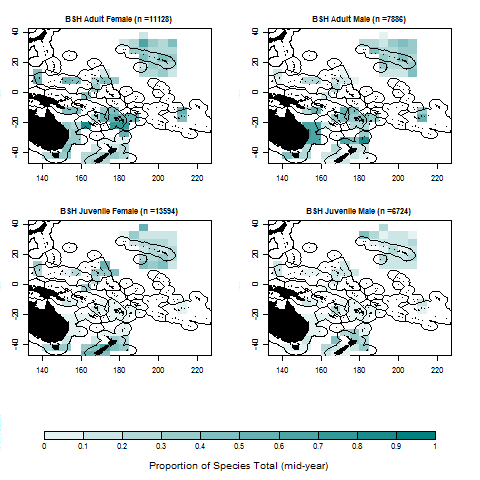
\includegraphics[width=\textwidth]{../GRAPHICS/Defined/BI_20_Map_maturity_sex_BSH_MY}
       \caption{Mid-year estimates.}
       \label{fig:test1}
   \end{subfigure}
   \begin{subfigure}[b]{0.6\textwidth}
       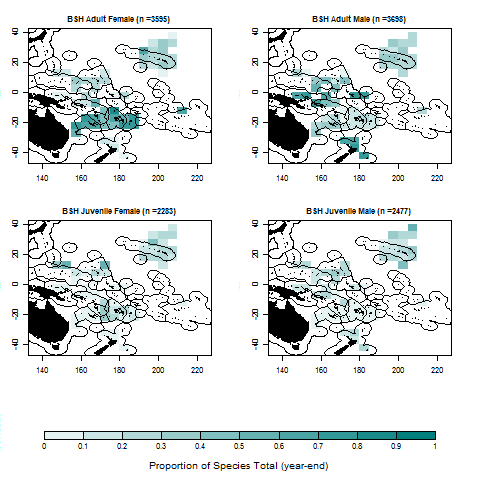
\includegraphics[width=\textwidth]{../GRAPHICS/Defined/BI_19_Map_maturity_sex_BSH}
       \caption{End of year estimates.}
       \label{fig:test2}
   \end{subfigure}
\caption{Blue Shark: Proportion of male and female as adults and juveniles in longline catches }
\label{fig:test} 
\end{figure}
\end{landscape}


%% Silky
\begin{landscape}
\begin{figure}
\centering
   \begin{subfigure}[b]{0.6\textwidth}
       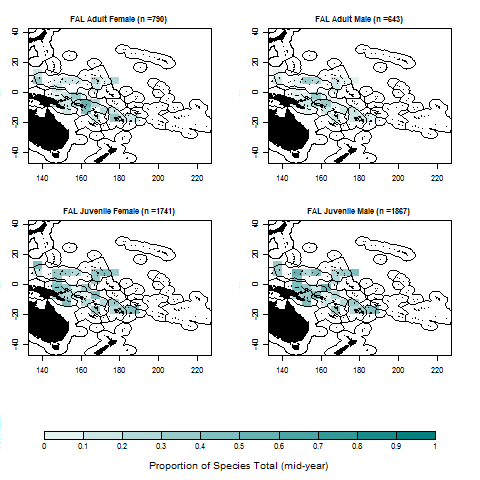
\includegraphics[width=\textwidth]{../GRAPHICS/Defined/BI_22_Map_maturity_sex_FAL_MY}
       \caption{Mid-year estimates.}
       \label{fig:test1}
   \end{subfigure}
   \begin{subfigure}[b]{0.6\textwidth}
       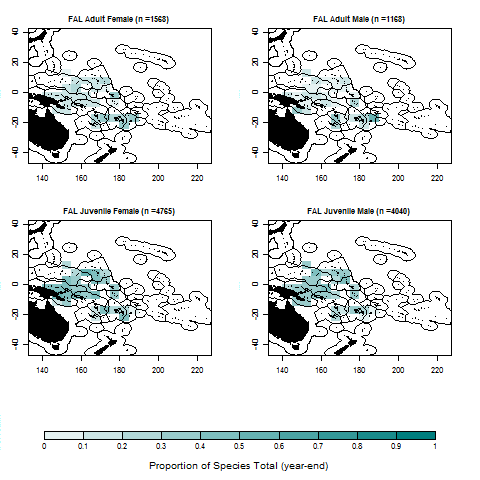
\includegraphics[width=\textwidth]{../GRAPHICS/Defined/BI_21_Map_maturity_sex_FAL}
       \caption{End of year estimates.}
       \label{fig:test2}
   \end{subfigure}
\caption{Silky Shark: Proportion of male and female as adult and juvenile in longline catches }
\label{fig:test} 
\end{figure}
\end{landscape}

%% Hammerhead
\begin{landscape}
\begin{figure}
\centering
   \begin{subfigure}[b]{0.6\textwidth}
       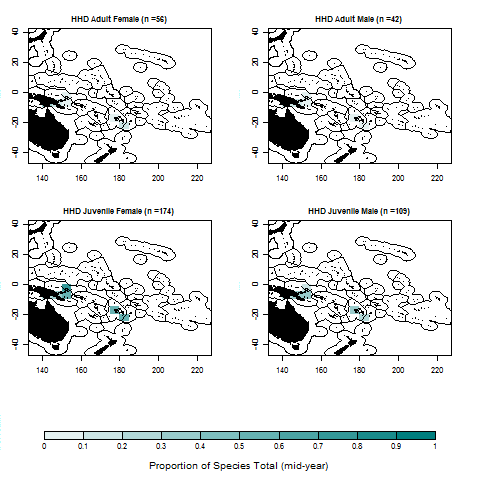
\includegraphics[width=\textwidth]{../GRAPHICS/Defined/BI_24_Map_maturity_sex_HHD_MY}
       \caption{Mid-year estimates.}
       \label{fig:test1}
   \end{subfigure}
   \begin{subfigure}[b]{0.6\textwidth}
       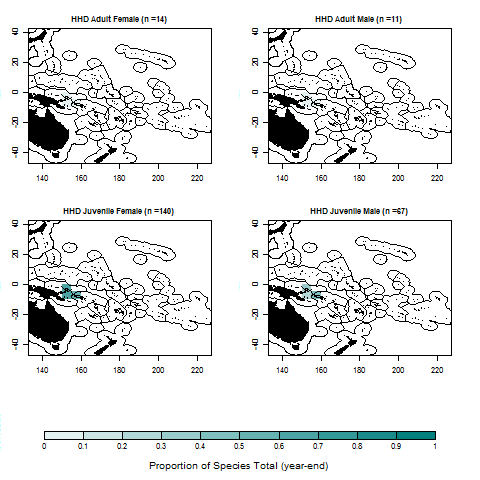
\includegraphics[width=\textwidth]{../GRAPHICS/Defined/BI_23_Map_maturity_sex_HHD}
       \caption{End of year estimates.}
       \label{fig:test2}
   \end{subfigure}
\caption{Hammerhead Shark: Proportion of male and female as adult and juvenile in longline catches }
\label{fig:test} 
\end{figure}
\end{landscape}

%% Mako
\begin{landscape}
\begin{figure}
\centering
   \begin{subfigure}[b]{0.6\textwidth}
       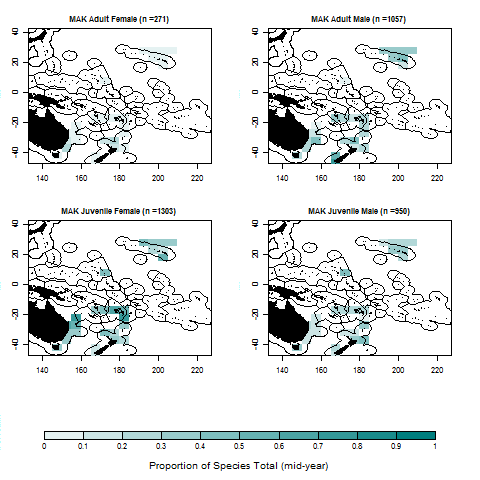
\includegraphics[width=\textwidth]{../GRAPHICS/Defined/BI_26_Map_maturity_sex_MAK_MY}
       \caption{Mid-year estimates.}
       \label{fig:test1}
   \end{subfigure}
   \begin{subfigure}[b]{0.6\textwidth}
       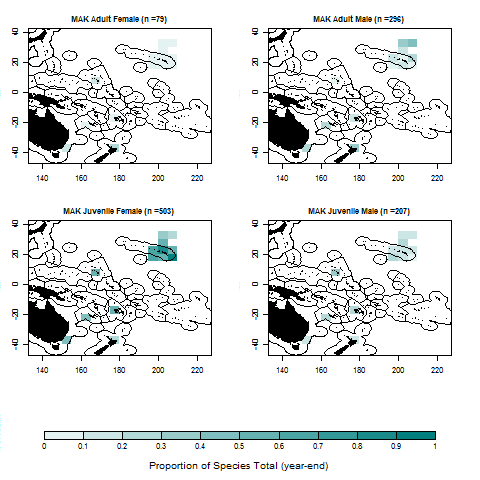
\includegraphics[width=\textwidth]{../GRAPHICS/Defined/BI_25_Map_maturity_sex_MAK}
       \caption{End of year estimates.}
       \label{fig:test2}
   \end{subfigure}
\caption{Mako Shark: Proportion of male and female as adult and juvenile in longline catches }
\label{fig:test} 
\end{figure}
\end{landscape}

%% OCS
\begin{landscape}
\begin{figure}
\centering
   \begin{subfigure}[b]{0.6\textwidth}
       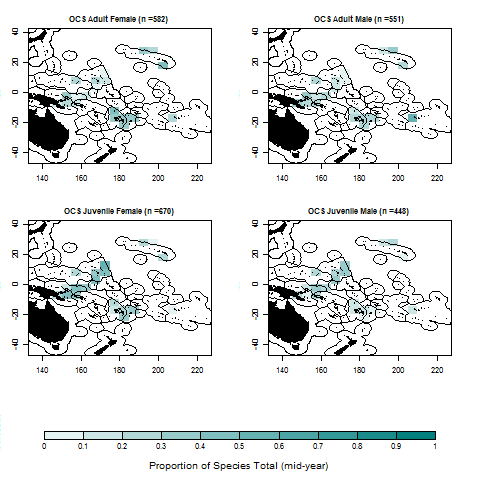
\includegraphics[width=\textwidth]{../GRAPHICS/Defined/BI_28_Map_maturity_sex_OCS_MY}
       \caption{Mid-year estimates.}
       \label{fig:test1}
   \end{subfigure}
   \begin{subfigure}[b]{0.6\textwidth}
       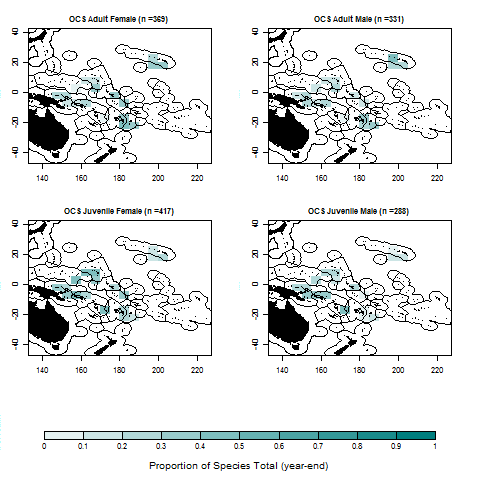
\includegraphics[width=\textwidth]{../GRAPHICS/Defined/BI_27_Map_maturity_sex_OCS}
       \caption{End of year estimates.}
       \label{fig:test2}
   \end{subfigure}
\caption{Oceanic Whitetip Shark: Proportion of male and female as adult and juvenile in longline catches }
\label{fig:test} 
\end{figure}
\end{landscape}

%% Porbeagle
\begin{landscape}
\begin{figure}
\centering
   \begin{subfigure}[b]{0.6\textwidth}
       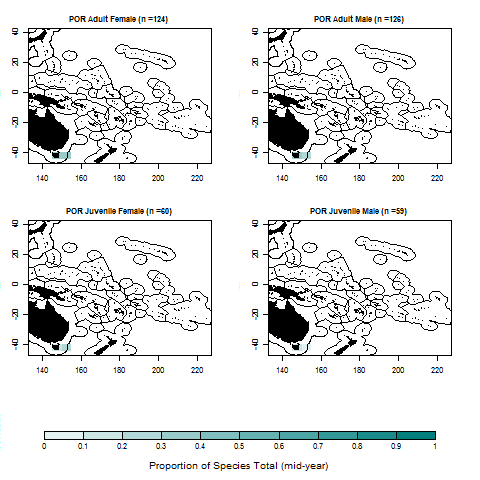
\includegraphics[width=\textwidth]{../GRAPHICS/Defined/BI_30_Map_maturity_sex_POR_MY}
       \caption{Mid-year estimates.}
       \label{fig:test1}
   \end{subfigure}
   \begin{subfigure}[b]{0.6\textwidth}
       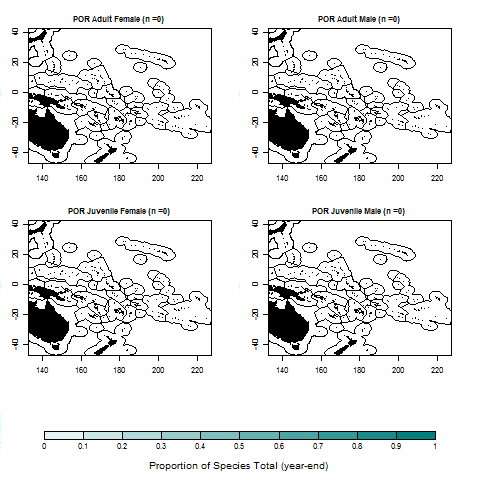
\includegraphics[width=\textwidth]{../GRAPHICS/Defined/BI_29_Map_maturity_sex_POR}
       \caption{End of year estimates.}
       \label{fig:test2}
   \end{subfigure}
\caption{Porbeagle Shark: Proportion of male and female as adult and juvenile in longline catches }
\label{fig:test} 
\end{figure}
\end{landscape}

%% Thresher
\begin{landscape}
\begin{figure}
\centering
   \begin{subfigure}[b]{0.6\textwidth}
       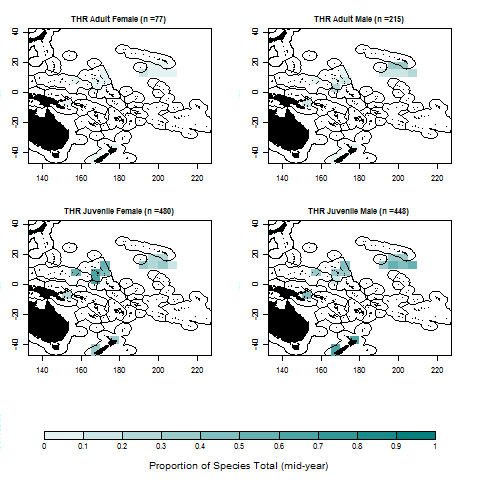
\includegraphics[width=\textwidth]{../GRAPHICS/Defined/BI_32_Map_maturity_sex_THR_MY}
       \caption{Mid-year estimates.}
       \label{fig:test1}
   \end{subfigure}
   \begin{subfigure}[b]{0.6\textwidth}
       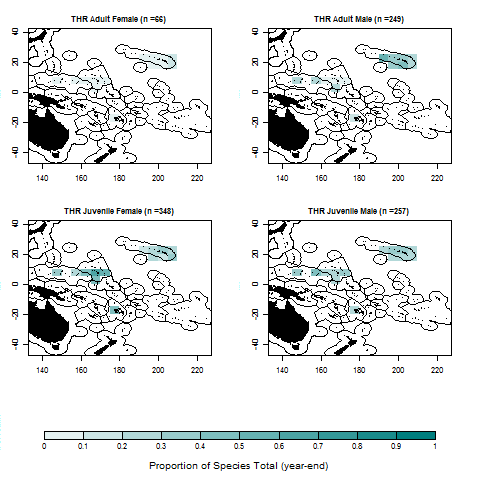
\includegraphics[width=\textwidth]{../GRAPHICS/Defined/BI_31_Map_maturity_sex_THR}
       \caption{End of year estimates.}
       \label{fig:test2}
   \end{subfigure}
\caption{Thresher Shark: Proportion of male and female as adult and juvenile in longline catches }
\label{fig:test} 
\end{figure}
\end{landscape}


%% UPPER JAW FORK LENGTH
\addcenterfig[Sex ratio (proportion female) of shark species caught by longline gear in the WCPO. The number of samples available for each sex and region is also shown.]{fig:map}{../GRAPHICS/Defined/BI_01_LLSexRatio_RDS}

\addcenterfig[Blue shark: median upper jaw fork length by year and region for males and females. Solid line shows median values, greyed area shows the limits of the 5th and 95th percentiles. The number of samples available for each sex and region is also shown.]{fig:map}{../GRAPHICS/Defined/BI_02_bio_len_BSH_RDS}

\addcenterfig[Silky shark: median upper jaw fork length by year and region for males and females. Solid line shows median values, greyed area shows the limits of the 5th and 95th percentiles. The number of samples available for each sex and region is also shown.]{fig:map}{../GRAPHICS/Defined/BI_03_bio_len_FAL_RDS}

\addcenterfig[Hammerhead shark: median upper jaw fork length by year and region for males and females. Solid line shows median values, greyed area shows the limits of the 5th and 95th percentiles. The number of samples available for each sex and region is also shown.]{fig:map}{../GRAPHICS/Defined/BI_04_bio_len_HHD_RDS}

\addcenterfig[Mako shark: median upper jaw fork length by year and region for males and females. Solid line shows median values, greyed area shows the limits of the 5th and 95th percentiles. The number of samples available for each sex and region is also shown.]{fig:map}{../GRAPHICS/Defined/BI_05_bio_len_MAK_RDS}

\addcenterfig[Oceanic Whitetip shark: median upper jaw fork length by year and region for males and females. Solid line shows median values, greyed area shows the limits of the 5th and 95th percentiles. The number of samples available for each sex and region is also shown.]{fig:map}{../GRAPHICS/Defined/BI_06_bio_len_OCS_RDS}

\addcenterfig[Porbeagle shark: median upper jaw fork length by year and region for males and females. Solid line shows median values, greyed area shows the limits of the 5th and 95th percentiles. The number of samples available for each sex and region is also shown.]{fig:map}{../GRAPHICS/Defined/BI_07_bio_len_POR_RDS}

\addcenterfig[Thresher shark: median upper jaw fork length by year and region for males and females. Solid line shows median values, greyed area shows the limits of the 5th and 95th percentiles. The number of samples available for each sex and region is also shown.]{fig:map}{../GRAPHICS/Defined/BI_08_bio_len_THR_RDS}


\addcenterfig[Silky shark: median upper jaw fork length by year and region for males and females caught by purse seine. Solid line shows median values, greyed area shows the limits of the 5th and 95th percentiles. The number of samples available for each sex and region is also shown.]{fig:map}{../GRAPHICS/Defined/BI_09_ps_bio_len_FAL}

\addcenterfig[Oceanic whitetip shark: median upper jaw fork length by year and region for males and females caught by purse seine. Solid line shows median values, greyed area shows the limits of the 5th and 95th percentiles. The number of samples available for each sex and region is also shown.]{fig:map}{../GRAPHICS/Defined/BI_10_ps_bio_len_OCS}


\clearpage


\addcenterfig[Blue shark: standardised length for male and females for longline data. Light grey line shows a lowess smoother.]{fig:map}{../GRAPHICS/Defined/BI_11_len_stdz_Blue_RDS}

\addcenterfig[Silky shark: standardised length for male and females for longline data. Light grey line shows a lowess smoother.]{fig:map}{../GRAPHICS/Defined/BI_12_len_stdz_Silky_RDS}

\addcenterfig[Hammerhead shark: standardised length for male and females for longline data. Light grey line shows a lowess smoother.]{fig:map}{../GRAPHICS/Defined/BI_13_len_stdz_Hammerhead_RDS}

\addcenterfig[Mako shark: standardised length for male and females. Light grey line shows a lowess smoother.]{fig:map}{../GRAPHICS/Defined/BI_14_len_stdz_Mako_RDS}

\addcenterfig[Oceanic Whitetip shark: standardised length for male and females for longline data. Light grey line shows a lowess smoother.]{fig:map}{../GRAPHICS/Defined/BI_15_len_stdz_OceanicWhiteTip}

\addcenterfig[Porbeagle shark: standardised length for male and females for longline data. Light grey line shows a lowess smoother.]{fig:map}{../GRAPHICS/Defined/BI_16_len_stdz_Porbeagle_RDS}

\addcenterfig[Thresher shark: standardised length for male and females for longline data. Light grey line shows a lowess smoother.]{fig:map}{../GRAPHICS/Defined/BI_17_len_stdz_Thresher_RDS}

\addcenterfig[Annual change in length (cm) over the study period as derived from the year effect of a GLM fitted to the sex and species specific data shown in figures 71 to 77 ]{fig:map}{../GRAPHICS/Defined/BI_18_len_stdz_coef_out}

\clearpage
\subsection{Management Considerations}

\addcenterfig[Fate of observed sharks caught by longline in the WCPO (total numbers for all species combined).]{fig:map}{../GRAPHICS/fate_ll_obs_by_region}

\addcenterfig[Fate of observed sharks caught by longline in the WCPO (proportion by number for all species combined).]{fig:map}{../GRAPHICS/fate_ll_ps_obs_all_keysharks_wcpo}


\addcenterfig[Fate of observed blue sharks caught by longline in the WCPO.]{fig:map}{../GRAPHICS/fate_ll_obs_BSH}
\addcenterfig[Fate of observed silky sharks caught by longline in the WCPO.]{fig:map}{../GRAPHICS/fate_ll_obs_FAL}
\addcenterfig[Fate of observed hammerhead sharks caught by longline in the WCPO.]{fig:map}{../GRAPHICS/fate_ll_obs_HHD}
\addcenterfig[Fate of observed mako sharks caught by longline in the WCPO.]{fig:map}{../GRAPHICS/fate_ll_obs_MAK}
\addcenterfig[Fate of observed oceanic whitetip sharks caught by longline in the WCPO.]{fig:map}{../GRAPHICS/fate_ll_obs_OCS}
\addcenterfig[Fate of observed porbeagle sharks caught by longline in the WCPO.]{fig:map}{../GRAPHICS/fate_ll_obs_POR}
\addcenterfig[Fate of observed thresher sharks caught by longline in the WCPO.]{fig:map}{../GRAPHICS/fate_ll_obs_THR}


\section{Model Diagnostics}
\subsubsection{CPUE Standardisation Diagnostics}

\addcenterfig[[CPUE indicators, model diagnostics for blue shark (north) CPUE standardization via negative binomial model.]{fig:map}{../GRAPHICS/BSH.north_MU~yy+program_code + HPBCAT2 + mm + sharkbait_SIGMA~program_code + HPBCAT2 + mm_resids}

\addcenterfig[[CPUE indicators, model diagnostics for blue shark (south) CPUE standardization via negative binomial model.]{fig:map}{../GRAPHICS/BSH.south_MU~yy+flag + HPBCAT2 + mm + sharkbait_SIGMA~intrcpt_resids}

\addcenterfig[[CPUE indicators, model diagnostics for silky shark CPUE standardization via negative binomial model.]{fig:map}{../GRAPHICS/FAL_MU~yy+program_code + HPBCAT2 + mm + sharkbait_SIGMA~program_code + sharkbait + mm_resids}

\addcenterfig[[CPUE indicators, model diagnostics for silky shark CPUE standardization via negative binomial model]{fig:map}{../GRAPHICS/HHD_MU~yy+program_code + HPBCAT2 + mm + sharkbait_SIGMA~sharkbait_resids}

\addcenterfig[[CPUE indicators, model diagnostics for silky shark CPUE standardization via negative binomial model.]{fig:map}{../GRAPHICS/MAK.north_MU~yy+program_code + mm + sharkbait_SIGMA~HPBCAT2_resids}

\addcenterfig[[CPUE indicators, model diagnostics for silky shark CPUE standardization via negative binomial model.]{fig:map}{../GRAPHICS/MAK.south_MU~yy+program_code + HPBCAT2 + mm + sharkbait_SIGMA~program_code + mm_resids}

\addcenterfig[[CPUE indicators, model diagnostics for silky shark CPUE standardization via negative binomial model.]{fig:map}{../GRAPHICS/OCS_MU~yy+program_code + HPBCAT2 + mm + sharkbait_SIGMA~program_code_resids}

\addcenterfig[f[CPUE indicators, model diagnostics for silky shark CPUE standardization via negative binomial model.]{fig:map}{../GRAPHICS/POR_MU~yy + flag + HPBCAT2 + mm_SIGMA~flag + mm_resids}

\addcenterfig[[CPUE indicators, model diagnostics for silky shark CPUE standardization via negative binomial model.]{fig:map}{../GRAPHICS/THR_MU~yy+program_code + HPBCAT2 + mm_SIGMA~HPBCAT2 + program_code_resids}

%\addcenterfig[CPUE indicators, nominal CPUE in the purse seine fishery, Unassociated Sets, Region 3.]{fig:cpue_ps_an1}{cpue_psnom_reg3_UNASS}
%\addcenterfig[CPUE indicators, nominal CPUE in the purse seine fishery, Unassociated sets, Region 4.]{fig:cpue_ps_an2}{cpue_psnom_reg4_UNASS}

%\addcenterfig[CPUE indicators, nominal CPUE in the purse seine fishery, Associated Sets, Region 3.]{fig:cpue_ps_an3}{cpue_psnom_reg3_assoc}
%\addcenterfig[CPUE indicators, nominal CPUE in the purse seine fishery, Associated sets, Region 4.]{fig:cpue_ps_an4}{cpue_psnom_reg4_assoc}

%----------------------------------------------------------------------------------------
 \subsubsection*{Blue Shark model diagnostics and extra plots}

%%%   Missing %\addcenterfig[CPUE indicators, GLM model diagnostics BSH in the North Pacific.]{fig:cpue_bsh_an1}{BSH_NB_N_diag}
  
  %\addcenterfig[CPUE indicators, GLM model diagnostics .]{fig:cpue_BSH_an2}{BSH_ZINB_S_diag}
  
  %\addcenterfig[CPUE indicators, GLM model diagnostics, BSH in the north Pacific step plot.]{fig:cpue_BSH_an3}{LLcpue_BSH_north_NB_step}
  %\addcenterfig[CPUE indicators, GLM model diagnostics, BSH in the south Pacific step plot.]{fig:cpue_BSH_an4}{ll_cpue_BSH_S_stepplot}
  
  
%-------------------------------------------------------------------   %~~~~~~~~~~~~~~~~ 
 
 
 %\addcenterfig[CPUE indicators, model diagnostics for mako shark CPUE standardization via negative binomial model, northern hemisphere.]{fig:cpue_MAK_an1}{LLcpue_MAK_north_NB_diag}
 %\addcenterfig[CPUE indicators, model diagnostics for mako shark CPUE standardization via negative binomial model, sourthern hemisphere.]{fig:cpue_MAK_an2}{LLcpue_MAK_south_NB_diag}
 
 
  %\addcenterfig[CPUE indicators, GLM model diagnostics, mako shark in the north Pacific step plot.]{fig:cpue_MAL_an3}{LLcpue_MAKO_north_NB_step}
  %\addcenterfig[CPUE indicators, step diagnostics for mako shark CPUE standardization via negative binomial model, sourthern hemisphere.]{fig:cpue_MAK_an4}{LLcpue_MAKO_south_NB_step}
 
 
 %-------------------------------------------------------------------
 \subsubsection*{Silky Shark model diagnostics and extra plots}
 
 %\addcenterfig.]{fig:cpue_fal_an1}{LLcpue_SILKY_NB_diag}
 %\addcenterfig[CPUE indicators, step plot for silky shark CPUE standardization via negative binomial model.]{fig:cpue_fal_an2}{LLcpue_FAL_NB_step}

%-------------------------------------------------------------------
\subsubsection*{Oceanic Whitetip Shark model diagnostics and extra plots}

 %\addcenterfig[CPUE indicators, model diagnostics for oceanic whitetip shark CPUE standardization via negative binomial model.]{fig:cpue_OCS_an1}{LLcpue_OCS_NB_diag}
 
  %\addcenterfig[CPUE indicators, stepplot for oceanic whitetip shark CPUE standardization via negative binomial model.]{fig:cpue_OCS_an2}{LLcpue_OCS_NB_step}
  
%-------------------------------------------------------------------
\subsubsection*{Thresher Shark model diagnostics and extra plots}

 %\addcenterfig[CPUE indicators, model diagnostics for thresher shark CPUE standardization via negative binomial model.]{fig:cpue_THR_an1}{LLcpue_THRESHER_NB_diag}
 %\addcenterfig[CPUE indicators, stepplot for thresher shark CPUE standardization via negative binomial model.]{fig:cpue_THR_an2}{LLcpue_THRESHER_NB_step}




%%%%%%%%%%%%%%%%%%%%%%%%%%%%%%%%%%%%%%%%%%
% SC Information Paper 5 
% SHARK INDICATORS IN THE WESTERN CENTRAL PACIFIC
% June 2015
%
% Author: Joel Rice (joelrice@uw.edu )
%
%
%%%%%%%%%%%%%%%%%%%%%%%%%%%%%%%%%%%%%%%%%

%----------------------------------------------------------------------------------------
%  PACKAGES AND OTHER DOCUMENT CONFIGURATIONS
%----------------------------------------------------------------------------------------



%\documentclass[12pt]{SCreport}

%\usepackage{fullpage}
\usepackage{amssymb, amsmath}
\usepackage{natbib}
\usepackage{booktabs}
\usepackage{url}
\usepackage{setspace}
\usepackage{hyperref}
%\usepackage{gensymb}
\usepackage{pdflscape}
\usepackage{etoolbox}
\usepackage[utf8]{inputenc}
\usepackage{graphicx}
\usepackage{caption}
\usepackage{parskip}
\usepackage[margin=1in]{geometry} % customize margins 
\usepackage{parskip} % one line between paragraphs
\usepackage{grffile} % allows ~, . ,etc. into figure file names

\usepackage{comment}
\usepackage[usenames,dvipsnames,svgnames]{xcolor}
\usepackage{soul}
\usepackage{xspace}


\onehalfspacing



% normal figure, centred in page
\newcommand{\capnow}{}
\newcommand{\addcenterfig}[3][Caption to be completed]{
  \begin{figure}[!h]
    \begin{center}
      \includegraphics[width=\textwidth]{#3}
     \caption{#1 \label{#2}}
    \end{center}
  \end{figure}
}

% landscape figure
\newcommand{\addcenterfigLS}[3][Caption to be completed]{
 \newgeometry{left=0.5cm,bottom=2.5cm,right=1cm,top=2.5cm}

\begin{landscape}
%\topskip0pt
   \vspace*{\fill}

\begin{figure}[!h]
    \begin{center}
      \includegraphics[width=620pt]{#3}
     \caption{#1 \label{#2}}
    \end{center}

  \end{figure}
  \vspace*{\fill}

\clearpage
\end{landscape}
\restoregeometry
}

%\graphicspath{ {C:/Projects/SHK-indicators-2015/GRAPHICS/}{C:/Projects/SHK-indicators-2015/GRAPHICS/CPUE_std/} }

%\usepackage[english]{babel}

%%%%%%%%%%%%%%%%%%%%%%%%%%%%%%%%%%%%%%%%%%%%%%%%%%%%%%%%%%%%%
%%%%%%%%%%%%%%%%%%%%% WCPFC title page %%%%%%%%%%%%%%%%%%%%% 
%% Commands for users to define title page settings
\newcommand{\spcauthor}{Use \textbackslash reportauthor to defined report authors}
\newcommand{\reportauthor}[1]{\renewcommand{\spcauthor}{#1}}

\newcommand{\spctitle}{Use \textbackslash reporttitle to defined report authors}
\newcommand{\reporttitle}[1]{\renewcommand{\spctitle}{#1}}

\newcommand{\repnumbr}{Use \textbackslash reportnumber to defined report authors}
\newcommand{\reportnumber}[1]{\renewcommand{\repnumbr}{#1}}

%% define title page macro 
\newcommand{\wcpfctitlepage}{

\thispagestyle{empty}
\begin{center}
\begin{figure}
\begin{center}

\includegraphics[scale=0.6]{WCPFC-logo.jpg}

\end{center}
\end{figure}
\textbf{SCIENTIFIC COMMITTEE\\ELEVENTH REGULAR SESSION\\}
Pohnpei, Federated States of Micronesia\\
5--13 August 2015\\

\vspace{0.5in}
\rule{\textwidth}{0.5mm}
%\vspace{-0.25cm}
\bfseries{\spctitle} % report title inserted here
\rule{\textwidth}{0.5mm}
\end{center}

\begin{flushright}
\textbf{WCPFC-SC11-2015/\repnumbr} % report number
\end{flushright}
\vspace{1in}

\begin{center} % report authors
\textbf{\spcauthor \footnote{\label{spc-ref}Oceanic Fisheries Programme, Secretariat of the Pacific Community}}
\end{center}

\clearpage}
%\reportauthor{Joel Rice\footnote{Joel Rice Consulting Ltd.}, Laura Tremblay-Boyer, and Shelton Harley}
%\reporttitle{Analysis of stock status and related indicators for key shark species of the Western Central Pacific Fisheries Commission}
%\reportnumber{SA-IP-05}



%----------------------------------------------------------------------------------------
%  Document content
%----------------------------------------------------------------------------------------

%\begin{document}

%----------------------------------------------------------------------------------------

\subsection{Longline Fishery Data}
%---------------------------------------------------------------------------------------------

\addcenterfig[Map of WCPO and observed effort. ]{fig:LLsets}{FIG_2_MAP_sets}

 
\addcenterfig[Total number of hooks fished by flag (for the top four fishing nations, and all others combined) based on   aggregated (5x5 degree square) data, for six regions of the WCPFC Statistical Area. ]{fig:LLLogbood_flag_hooks}{FIG_xx_LLeff_FLAG}
 

\addcenterfig[Total number of reported sharks  by flag (for the top four fishing nations, and all others combined) based aggregated (5x5 degree square) data, for six regions of the WCPFC Statistical Area.]{fig:LLLog_flag_shks}{FIG_xx_LLreported_catch_FLAG}
 

\addcenterfig[Total number of hooks observed by flag (for the top four fishing nations) based on longline observer records held by the SPC-OFP, for six regions of the WCPFC Statistical Area  ]{fig:obsLL_flag}{FIG_xx_LLeff_FLAG}    

\addcenterfig[Logsheet effort by month.]{fig:logeffmnth}{FIG_xx_LOGSHEET_mm}
\addcenterfig[Observed effort by month.]{fig:obseffmnth}{FIG_xx_obsBY_mm}
\addcenterfig[Absolute percent difference in effort between reported (logsheet)  effort and observed effort.]{fig:effdiff}{FIG_xx_obsDIFFlog_mm}


\clearpage

              
\addcenterfig[Aggregate effort by region. ]{fig:aggeff}{FIG_xx_agg_eff}
%\addcenterfig[Observed effort by region.]{fig:obseff}{FIG_xx_OBS_eff}

\addcenterfig[Observed purse seine in the  WCPO showing the top four fishing nations and all others combined.  ]{fig:pssets}{FIG_xx_PS_eMAP_sets}

%-------------------------------------------------------------------------------------------------------------------------
 
 \subsubsection*{Fishing Effort- Purse Seine} 
 
 \addcenterfig[Absolute percent difference in effort between reported (logsheet)  effort and observed effort.]{fig:seine_map}{FIG_xx_PS_sets}
 
 
 \addcenterfig[Comparison by region and flag of purse seine effort (in sets) associated sets using aggregated (5x5 degree square) data for six regions of the WCPFC Statistical Area, excluding data from Indonesia, Vietnam, and Japan coastal waters.]{fig:ps_ass_eff}{ps_total_effAssociated}
  \addcenterfig[Comparison by region and flag of purse seine effort (in sets) unassociated sets using aggregated (5x5 degree square) data for six regions of the WCPFC Statistical Area, excluding data from Indonesia, Vietnam, and Japan coastal waters.]{fig:ps_una_eff}{ps_total_effUnassociated} 

 \addcenterfig[Total sharks recorded on logsheets (in number of sets recording at least one shark interaction), for associated sets.]{fig:log_ass_shk}{ps_oper_shks_rep_cntry_associated}
 \addcenterfig[Total sharks recorded on logsheets (in number of sets recording at least one shark interaction), for unassociated sets.]{fig:log_una_shk}{ps_oper_shks_rep_cntry_unassociated} 
 
 
 
 
\clearpage         
 %       \subsection{Data formatting}
 %       \subsection{Limitations - Caveats}
        
        
%----------------------------------------------------------------------------------------
%  Distribuion Indicators
%----------------------------------------------------------------------------------------
             
        
\section{Distribution Indicator Analyses}
      \subsection{Introduction}
      \subsection{Methods}
      \subsection{Results}
         

\clearpage         
%----------------------------------------------------------------------------------------
          \subsubsection{Blue Shark}

\addcenterfig[Blue shark distribution indicators. Proportion of positive sets, observer data.]{fig:bsh1}{FIG_xx_pcntpos_reg_BSH}
\addcenterfig[Blue shark distribution indicators. Proportion of 5 degree squares having CPUE greater than 1 per 1000 hooks region, observer data.]{fig:bsh2}{FIG_xx_HIGH_CPUE_BSH}


%----------------------------------------------------------------------------------------
\subsubsection{Mako Shark}

\addcenterfig[Mako shark distribution indicators. Proportion of positive sets, observer data.]{fig:mak1}{FIG_xx_pcntpos_reg_MAK}          
\addcenterfig[Mako shark distribution indicators. Proportion of 5 degree squares having CPUE greater than 1 per 1000 hooks region, observer data.]{fig:mak2}{FIG_xx_HIGH_CPUE_MAK}
          
          
%----------------------------------------------------------------------------------------
 \subsubsection{Silky Shark}
 
\addcenterfig[Mako shark distribution indicators. Proportion of positive sets, observer data.]{fig:fal1}{FIG_xx_pcntpos_reg_FAL}           
\addcenterfig[Silky shark distribution indicators. Proportion of 5 degree squares having CPUE greater than 1 per 1000 hooks region, observer data.]{fig:fal2}{FIG_xx_HIGH_CPUE_FAL}

%----------------------------------------------------------------------------------------
 \subsubsection{Oceanic Whitetip Shark}
 \addcenterfig[Oceanic whitetip shark distribution indicators. Proportion of positive sets, observer data.]{fig:ocs1}{FIG_xx_pcntpos_reg_OCS}          
 \addcenterfig[Oceanic whitetip shark distribution indicators. Proportion of 5 degree squares having CPUE greater than 1 per 1000 hooks region, observer data.]{fig:ocs2}{FIG_xx_HIGH_CPUE_OCS}

%----------------------------------------------------------------------------------------
 \subsubsection{Thresher Shark}
\addcenterfig[Thresher shark distribution indicators. Proportion of positive sets, observer data.]{fig:thr1}{FIG_xx_pcntpos_reg_THR} 
\addcenterfig[Thresher shark distribution indicators. Proportion of 5 degree squares having CPUE greater than 1 per 1000 hooks region, observer data.]{fig:thr2}{FIG_xx_HIGH_CPUE_THR}
          
%----------------------------------------------------------------------------------------
 \subsubsection{Hammerhead Shark}
\addcenterfig[Hammerhead shark distribution indicators. Proportion of positive sets, observer data.]{fig:HHD1}{FIG_xx_pcntpos_reg_HHD} 
\addcenterfig[Hammerhead shark distribution indicators. Proportion of 5 degree squares having CPUE greater than 1 per 1000 hooks region, observer data.]{fig:HHD2}{FIG_xx_HIGH_CPUE_HHD}

%----------------------------------------------------------------------------------------
\subsubsection{Porbeagle Shark}
\addcenterfig[Porbeagle shark distribution indicators. Proportion of positive sets, observer data.]{fig:POR1}{FIG_xx_pcntpos_reg_POR} 
\addcenterfig[Porbeagle shark distribution indicators. Proportion of 5 degree squares having CPUE greater than 1 per 1000 hooks region, observer data.]{fig:POR2}{FIG_xx_HIGH_CPUE_POR}

  \subsection{Conclusions}
%----------------------------------------------------------------------------------------
%  Species COmposition
%----------------------------------------------------------------------------------------
      
      
\section{Observed Species Composition Indicator Analyses}
      \subsection{Introduction}
      \subsection{Methods}
      \subsection{Results}
      
  \subsubsection*{Longline}      
  \addcenterfig[Catch Composition Indicators. Sharks Per. 1000 hooks by region, observer data.]{fig:catchcomp1}{FIG_xx_shksP1000Hooks}
  \addcenterfig[Catch Composition Indicators. Sharks Per. 1000 hooks by region, deep sets observer data.]{fig:catchcomp2}{FIG_xx_shksP1000Hooks_deep}  
  \addcenterfig[Catch Composition Indicators. Sharks Per. 1000 hooks by region, shallow sets observer data.]{fig:catchcomp3}{FIG_xx_shksP1000Hooks_shallow}
  \addcenterfig[Catch Composition Indicators. Proportional catch of main species and other sharks by retions.]{fig:catchcomp3a}{catchcomp_xx_llshks_pcnt}
  
  
%------------------------------------------------------------------------------------------
\clearpage
 \subsubsection*{Purse Seine}        
 \addcenterfig[Catch Composition Indicators. Sharks per set, observer data.]{fig:catchcomp4}{FIG_xx_PS_shks_set}
 \addcenterfig[Catch Composition Indicators. Sharks per set, associated sets, observer data]{fig:catchcomp5}{FIG_xx_PS_shks_UNAS}  
 \addcenterfig[Catch Composition Indicators. Sharks per set, unassociated sets, observer data.]{fig:catchcomp6}{FIG_xx_PS_shks_ASSO} 

  \addcenterfig[Catch Composition Indicators. Catch composition by proportion , observer data.]{fig:catchcomp7}{catchcomp_xx_PS_comp_reg}
 \addcenterfig[Catch Composition Indicators. Catch composition by proportion, associated sets, observer data]{fig:catchcomp8}{catchcomp_xx_PS_comp_reg_UNAS}  
 \addcenterfig[Catch Composition Indicators. Catch composition by proportion, unassociated sets, observer data.]{fig:catchcomp9}{catchcomp_xx_PS_comp_reg_ASSOC} 

 
 
 \subsection{Conclusions}
      
      
 \clearpage          

%----------------------------------------------------------------------------------------
%  CPUE INDICATORS
%----------------------------------------------------------------------------------------
\section{Catch Per Unit Effort indicator analyses}

\subsection*{Purse Seine data preparation}

\addcenterfig[CPUE indicators, nominal CPUE in the purse seine fishery, all sets, Region 3.]{fig:cpue_ps1}{cpue_psnom_reg3}
\addcenterfig[CPUE indicators, nominal CPUE in the purse seine fishery, all sets, Region 4.]{fig:cpue_ps2}{cpue_psnom_reg4}






%----------------------------------------------------------------------------------------
%----------------------------------------------------------------------------------------
\clearpage  
\subsection{Results}
    %----------------------------------------------------------------------------------------

  \subsubsection{Blue Shark}
           
\addcenterfig[Blue shark CPUE indicators. Proportion of positive sets, observer data.]{fig:bshcp1}{FIG_xx_pcntpos_reg_BSH}
\addcenterfig[Blue shark CPUE indicators. Nominal CPUE, sharks per 1000 hooks, observer data.]{fig:bshcp2}{FIG_xx_nomCPUE_reg_BSH}


% \addcenterfig[Blue shark CPUE indicators. Standardized blue shark CPUE based on the negative binomial model for observer data in the northern hemisphere.]{fig:bshcp3}{LLcpue_BSH_north_NB_step}
% 
% \addcenterfig[Blue shark CPUE indicators. Standardized CPUE, zero inflated negative binomial Southern Hemisphere, observer data.]{fig:bshcp4}{ll_cpue_BSHzinb_nominal}
% 
%  



%----------------------------------------------------------------------------------------
 \subsubsection{Mako Shark}
%           
 \addcenterfig[Mako shark CPUE indicators. Proportion of positive sets, observer data.]{fig:makcp1}{FIG_xx_pcntpos_reg_MAK}
  \addcenterfig[Mako shark CPUE indicators. Nominal CPUE, sharks per 1000 hooks, observer data.]{fig:makcp2}{FIG_xx_nomCPUE_reg_MAK}
% 
% \addcenterfig[Mako shark CPUE indicators. Standardized CPUE, mako shark in the northern hemisphere.]{fig:makcp3}{LLcpue_MAKO_north_NB_cpue}
% \addcenterfig[Mako shark CPUE indicators. Standardized CPUE, mako shark in the southern hemisphere.]{fig:makcp4}{LLcpue_MAKO_southth_NB_cpue}


\clearpage
%----------------------------------------------------------------------------------------
\subsubsection{Silky Shark}

  \addcenterfig[Silky shark CPUE indicators. Proportion of positive sets, observer data.]{fig:falcp1}{FIG_xx_pcntpos_reg_FAL}
 \addcenterfig[Silky shark CPUE indicators. Nominal CPUE, sharks per 1000 hooks, observer data.]{fig:falcp2}{FIG_xx_nomCPUE_reg_FAL}
% \addcenterfig[Silky shark CPUE indicators. Standardized CPUE from longline observer data for silky sharks.]{fig:falcp3}{LLcpue_FAL_NB_cpue}



%----------------------------------------------------------------------------------------
\subsubsection{Oceanic Whitetip Shark}
%           
 \addcenterfig[Oceanic whitetip shark CPUE indicators. Proportion of positive sets, observer data.]{fig:ocscp1}{FIG_xx_pcntpos_reg_OCS}
 \addcenterfig[Oceanic whitetip shark CPUE indicators. Nominal CPUE, sharks per 1000 hooks, observer data.]{fig:ocscp2}{FIG_xx_nomCPUE_reg_OCS}
% \addcenterfig[Oceanic whitetip shark CPUE indicators. Standardized CPUE based on negative  binomial models applied to observer data.]{fig:ocscp3}LLcpue_OCS_NB_cpue}


%----------------------------------------------------------------------------------------
  \subsubsection{Thresher Shark}
          
 \addcenterfig[Thresher shark CPUE indicators. Proportion of positive sets, observer data.]{fig:thrcp1}{FIG_xx_pcntpos_reg_THR}
 \addcenterfig[Thresher shark CPUE indicators. Nominal CPUE, sharks per 1000 hooks, observer data.]{fig:thrcp2}{FIG_xx_nomCPUE_reg_THR}
% \addcenterfig[Thresher shark CPUE indicators.  Standardized CPUE of thresher shark based on longline observer data.]{fig:thrcp3}{LLcpue_THRESHER_NB_cpue}


%----------------------------------------------------------------------------------------          
%----------------------------------------------------------------------------------------
  \subsubsection{Hammerhead Shark}
          
 \addcenterfig[Thresher shark CPUE indicators. Proportion of positive sets, observer data.]{fig:HHDcp1}{ }
 \addcenterfig[Thresher shark CPUE indicators. Nominal CPUE, sharks per 1000 hooks, observer data.]{fig:HHDcp2}{ }
% \addcenterfig[Thresher shark CPUE indicators.  Standardized CPUE of thresher shark based on longline observer data.]{fig:thrcp3}{LLcpue_THRESHER_NB_cpue}
   
     \subsubsection{Hammerhead Shark}
          
 \addcenterfig[Thresher shark CPUE indicators. Proportion of positive sets, observer data.]{fig:HHDcp1}{ }
 \addcenterfig[Thresher shark CPUE indicators. Nominal CPUE, sharks per 1000 hooks, observer data.]{fig:HHDcp2}{ }
% \addcenterfig[Thresher shark CPUE indicators.  Standardized CPUE of thresher shark based on longline observer data.]{fig:thrcp3}{LLcpue_THRESHER_NB_cpue}
      
   
 \clearpage     
      
      
      
      
     
%----------------------------------------------------------------------------------------
%  Biological
%----------------------------------------------------------------------------------------
      
\section{Biological indicator analyses}
     
      
%----------------------------------------------------------------------------------------
%  Discussion Type Sections.........
%----------------------------------------------------------------------------------------
         
      
\section{Feasibility of Stock Assessments}
\section{Impact of Recent Shark Management Measures}
 % analysis of fate and condition goes here? 

\section{Recommendations for Future Indicator Work}
\section{Management Implications}

\section*{Acknowledgements}
\clearpage
%----------------------------------------------------------------------------------------
%  REFERENCE LIST
%----------------------------------------------------------------------------------------


%----------------------------------------------------------------------------------------
%  Appendices 
%----------------------------------------------------------------------------------------

\section{Appendices}
% 
\subsection{CPUE Indicators.  Model diagnostics and extra plots}

% \addcenterfig[CPUE indicators, nominal CPUE in the purse seine fishery, Unassociated Sets, Region 3.]{fig:cpue_ps_an1}{cpue_psnom_reg3_UNASS}
% \addcenterfig[CPUE indicators, nominal CPUE in the purse seine fishery, Unassociated sets, Region 4.]{fig:cpue_ps_an2}{cpue_psnom_reg4_UNASS}
% 
% \addcenterfig[CPUE indicators, nominal CPUE in the purse seine fishery, Associated Sets, Region 3.]{fig:cpue_ps_an3}{cpue_psnom_reg3_assoc}
% \addcenterfig[CPUE indicators, nominal CPUE in the purse seine fishery, Associated sets, Region 4.]{fig:cpue_ps_an4}{cpue_psnom_reg4_assoc}

%----------------------------------------------------------------------------------------
 \subsubsection*{Blue Shark model diagnostics and extra plots}

%%%   Missing \addcenterfig[CPUE indicators, GLM model diagnostics BSH in the North Pacific.]{fig:cpue_bsh_an1}{BSH_NB_N_diag}
%   
%   \addcenterfig[CPUE indicators, GLM model diagnostics .]{fig:cpue_BSH_an2}{BSH_ZINB_S_diag}
%   
%   \addcenterfig[CPUE indicators, GLM model diagnostics, BSH in the north Pacific step plot.]{fig:cpue_BSH_an3}{LLcpue_BSH_north_NB_step}
%   \addcenterfig[CPUE indicators, GLM model diagnostics, BSH in the south Pacific step plot.]{fig:cpue_BSH_an4}{ll_cpue_BSH_S_stepplot}
%   
%   
%-------------------------------------------------------------------   %~~~~~~~~~~~~~~~~ 
 
 
%  \addcenterfig[CPUE indicators, model diagnostics for mako shark CPUE standardization via negative binomial model, northern hemisphere.]{fig:cpue_MAK_an1}{LLcpue_MAK_north_NB_diag}
%  \addcenterfig[CPUE indicators, model diagnostics for mako shark CPUE standardization via negative binomial model, sourthern hemisphere.]{fig:cpue_MAK_an2}{LLcpue_MAK_south_NB_diag}
%  
%  
%   \addcenterfig[CPUE indicators, GLM model diagnostics, mako shark in the north Pacific step plot.]{fig:cpue_MAL_an3}{LLcpue_MAKO_north_NB_step}
%  \addcenterfig[CPUE indicators, step diagnostics for mako shark CPUE standardization via negative binomial model, sourthern hemisphere.]{fig:cpue_MAK_an4}{LLcpue_MAKO_south_NB_step}
%  
 
 %-------------------------------------------------------------------
 \subsubsection*{Silky Shark model diagnostics and extra plots}
 
%  \addcenterfig[CPUE indicators, model diagnostics for silky shark CPUE standardization via negative binomial model.]{fig:cpue_fal_an1}{LLcpue_SILKY_NB_diag}
%  
%   \addcenterfig[CPUE indicators, step plot for silky shark CPUE standardization via negative binomial model.]{fig:cpue_fal_an2}{LLcpue_FAL_NB_step}

%-------------------------------------------------------------------
\subsubsection*{Oceanic Whitetip Shark model diagnostics and extra plots}

%  \addcenterfig[CPUE indicators, model diagnostics for oceanic whitetip shark CPUE standardization via negative binomial model.]{fig:cpue_OCS_an1}{LLcpue_OCS_NB_diag}
%  
%   \addcenterfig[CPUE indicators, stepplot for oceanic whitetip shark CPUE standardization via negative binomial model.]{fig:cpue_OCS_an2}{LLcpue_OCS_NB_step}
  
%-------------------------------------------------------------------
\subsubsection*{Thresher Shark model diagnostics and extra plots}
% 
%  %\addcenterfig[CPUE indicators, model diagnostics for thresher shark CPUE standardization via negative binomial model.]{fig:cpue_THR_an1}{LLcpue_THR_NB_diag}
%  %\addcenterfig[CPUE indicators, stepplot for thresher shark CPUE standardization via negative binomial model.]{fig:cpue_THR_an2}{LLcpue_THR_NB_step}
% 
%   \addcenterfig[CPUE indicators, model diagnostics for thresher shark CPUE standardization via negative binomial model.]{fig:cpue_THR_an1}{LLcpue_THRESHER_NB_diag}
%  \addcenterfig[CPUE indicators, stepplot for thresher shark CPUE standardization via negative binomial model.]{fig:cpue_THR_an2}{LLcpue_THRESHER_NB_step}

%-------------------------------------------------------------------
\clearpage
\subsubsection*{Species Distribution Maps}

 \addcenterfig[Species distribution, blue shark observed in the longline fishery.]{fig:dist_map_bsh}{LL_spec_dist_BSH}
  \addcenterfig[Species distribution, blue shark observed in the longline fishery by observer program.]{fig:obs_map_bsh}{obs-data-shk-catch-program_blue.png}
 \addcenterfig[Species distribution, silky shark observed in the longline fishery.]{fig:dist_map_fal}{LL_spec_dist_FAL}
   \addcenterfig[Species distribution, blue shark observed in the longline fishery by observer program.]{fig:obs_map_silky}{obs-data-shk-catch-program_silky.png}
 \addcenterfig[Species distribution, mako shark observed in the longline fishery.]{fig:dist_map_mak}{LL_spec_dist_mak}
   \addcenterfig[Species distribution, blue shark observed in the longline fishery by observer program.]{fig:obs_map_mako}{obs-data-shk-catch-program_mako.png}
 \addcenterfig[Species distribution, oceanic whitetip shark observed in the longline fishery.]{fig:dist_map_OCS}{LL_spec_dist_OCS}
   \addcenterfig[Species distribution, blue shark observed in the longline fishery by observer program.]{fig:obs_map_ocs}{obs-data-shk-catch-program_ocs.png}
 \addcenterfig[Species distribution, thresher shark observed in the longline fishery.]{fig:dist_map_THR}{LL_spec_dist_THR}
   \addcenterfig[Species distribution, blue shark observed in the longline fishery by observer program.]{fig:obs_map_thresher}{obs-data-shk-catch-program_thresher.png}
   \addcenterfig[Species distribuion, hammerhead shark observed in the longline fishery.]{fig:dist_map_HHD}{LL_spec_dist_HHD}
  \addcenterfig[Species distribuion, porbeagle shark observed in the longline fishery.]{fig:dist_map_POR}{LL_spec_dist_POR}


 
%-------------------------------------------------------------------
%-------------------------------------------------------------------
%-------------------------------------------------------------------


      
\end{document}




%-------------------------------------------------------------------
%-------------------------------------------------------------------
%-------------------------------------------------------------------

\end{document}



